\section{SRAM Architecture}
\label{arch}
ViPro assumes a single-bank architecture (Figure~\ref{fig:arch}),with a conventional 6T bitcell. The model used for determining the energy per access and minimum cycle time is based on this architecture. Larger memory capacities are usually organized in a multiple bank architecture, which is out of the scope of the current implementation of ViPro. Each SRAM component in the single-bank architecture is described below in the following sub-sections.

\begin{figure}[htb]
  \centering
  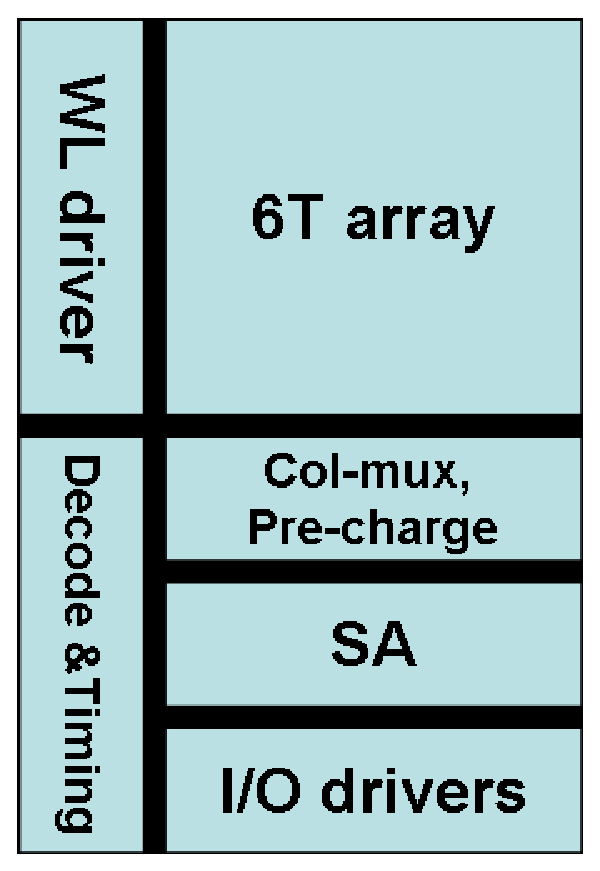
\includegraphics[scale=0.5]{Vipro_arch}
\vspace{-5pt}
  \caption{Single-bank SRAM architecture assumed by ViPro.}
  \label{fig:arch}
\vspace{-5pt}
\end{figure}

\subsection{Decoders and WL Driver}
The WL Driver assumed by ViPro (Figure~\ref{fig:wld})is a generic via-programmable circuit that can drive 8 WLs. It consits of a 2-input And, a 2-input Nand, and an inverter that drives the WL to the bitcells. The  Nand and And gates combine the pre-decoded signals to select a single WL. By connecting the inputs of the And gate to different combinations of the pre-decode signals (PRE8\_6 and PRE5\_3), different sets of 8 WLs can be driven. This structure enables only a single pre-decode (3 to 8) in the timing block (Figure~\ref{fig:tmg}) to be used for any number of rows, narrowing the optimization problem for the decoder to a single structure. The programmability of the WL driver also has potential benefits for schematic and layout automation.

\begin{figure}[htb]
  \centering
  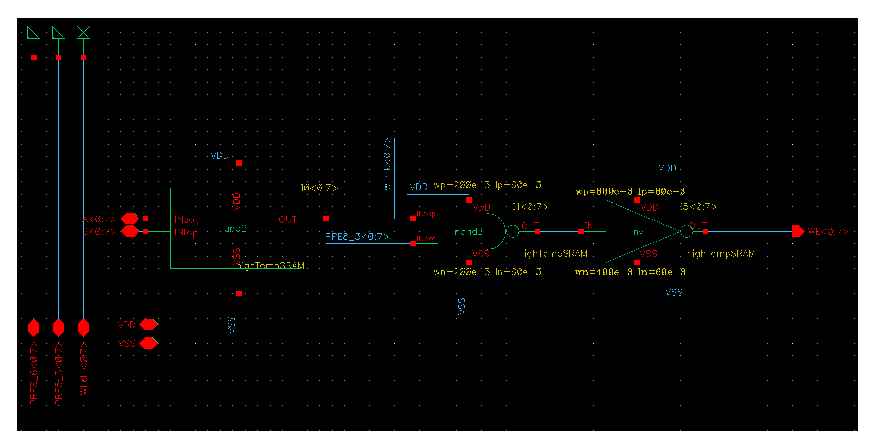
\includegraphics[scale=0.7]{WLD}
\vspace{-5pt}
  \caption{Via-programmable wordline driver in the ViPro architecture (zoom in for a clearer view).}
  \label{fig:wld}
\vspace{-5pt}
\end{figure}

\begin{figure}[htb]
  \centering
  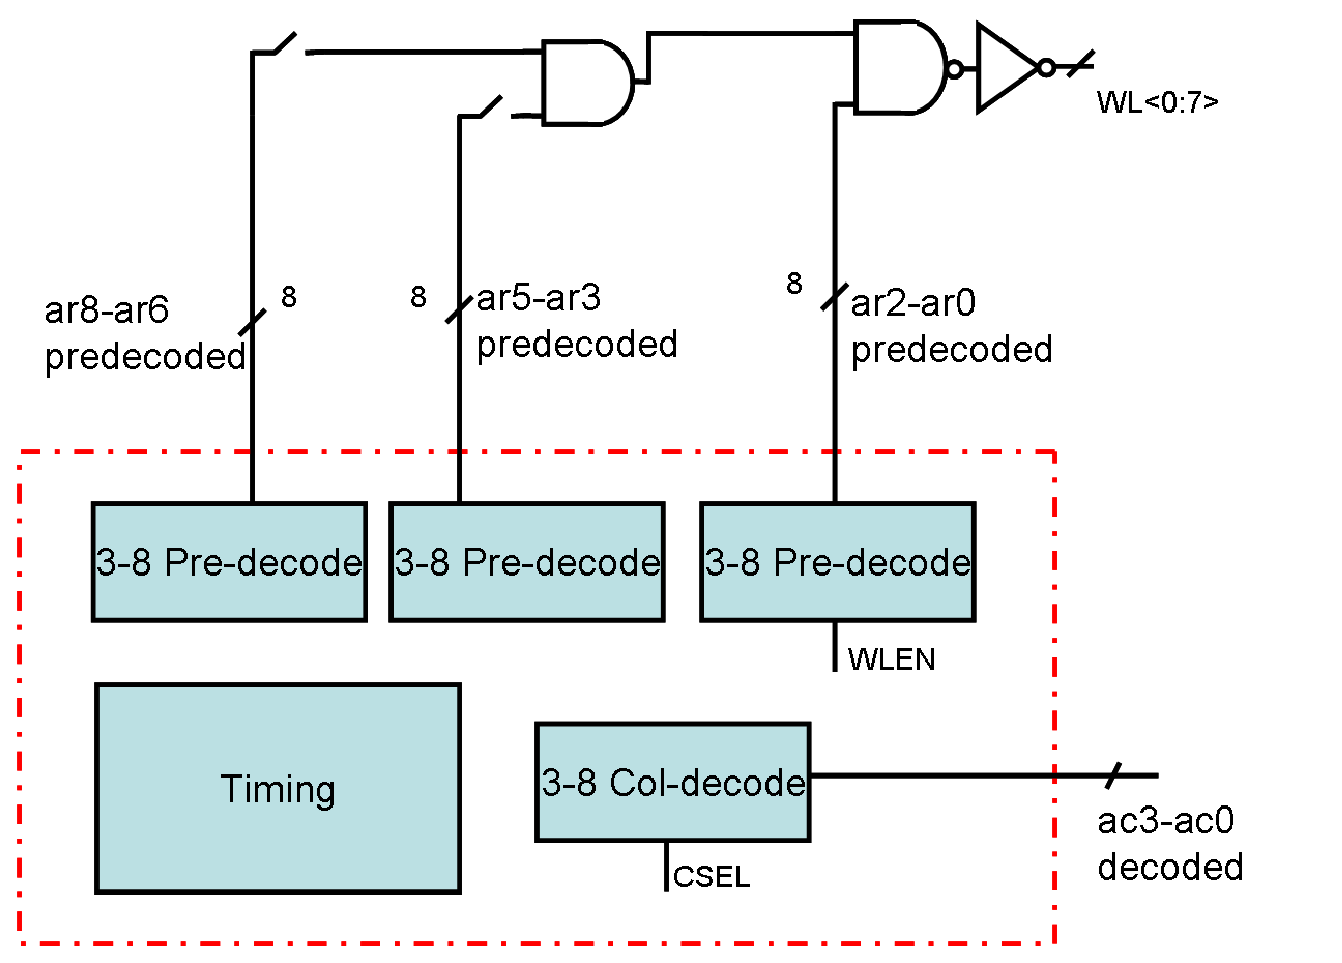
\includegraphics[scale=0.5]{Vipro_row}
\vspace{-5pt}
  \caption{Timing block showing the predecode and the WL Driver.}
  \label{fig:tmg}
\vspace{-5pt}
\end{figure}

\subsection{CD}
The CD (Figure~\ref{fig:cd}) is composed of the BL precharge and equalize transistors, and the column-mux transmisssion gate. The figure shows a CD that uses a column-mux of 4. In general, a larger column-mux (e.g. 8) can be used for all cases, with the unused outputs of the decoder left floating. This also narrows the optimization problem.
\begin{figure}[htb]
  \centering
  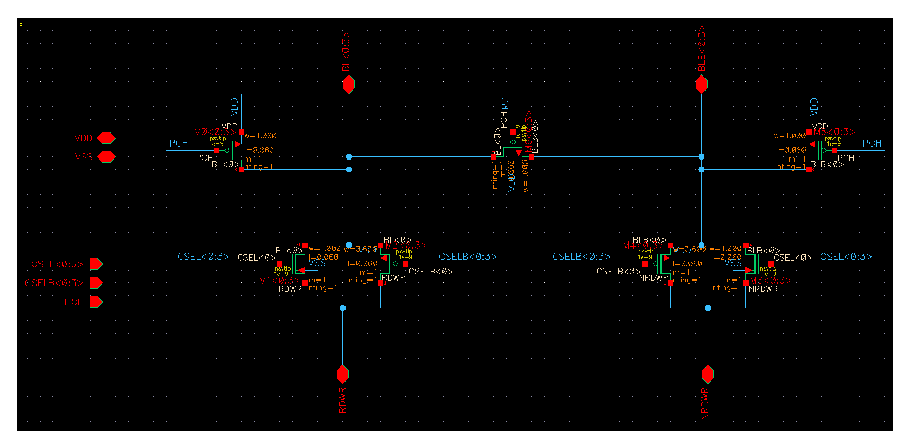
\includegraphics[scale=0.8]{CD}
\vspace{-5pt}
  \caption{Column Mux circuit.}
  \label{fig:cd}
\vspace{-5pt}
\end{figure}


\subsection{SA}
The SA (Figure~\ref{fig:sa}) is composed of a differential voltage SA, a nand-based SR output latch, and precharge and equalize PFETS for the SA input nodes -  the muxed-out BLs (RDWR and NRDWR). The SA inputs are also connected to the write drivers (tri-state inverters) in the IO circuit.

\begin{figure}[htb]
  \centering
  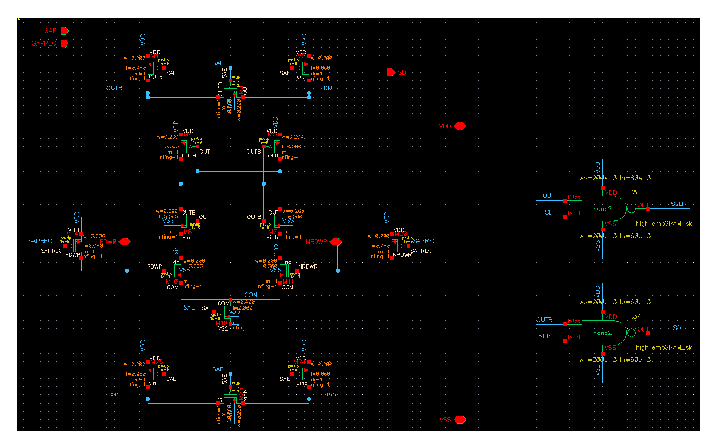
\includegraphics[scale=1.0]{SA}
\vspace{-5pt}
  \caption{Sense Amp circuit.}
  \label{fig:sa}
\vspace{-5pt}
\end{figure}

\subsection{IO}
The IO (Figure~\ref{fig:io}) consists of a flip-flop for the SA output during a read, and another one for the data input during a write. It also has tri-state inverters to drive the data to the bitlines, that get enabled during a write.

\begin{figure}[htb]
  \centering
  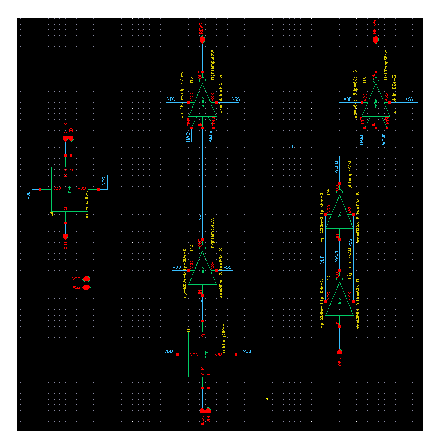
\includegraphics[scale=0.7]{IO}
\vspace{-5pt}
  \caption{Data Input and Output driver circuits. }
  \label{fig:io}
\vspace{-5pt}
\end{figure}

\subsection{Timing}
The precise timing block design varies from technology to technology depending on design constraints, capacitance of the control wires that need to be driven, etc. The basic functionality of the timing block and the control signals it drives is captured in Figure~\ref{fig:tmgblk}. 

\begin{figure}[htb]
  \centering
  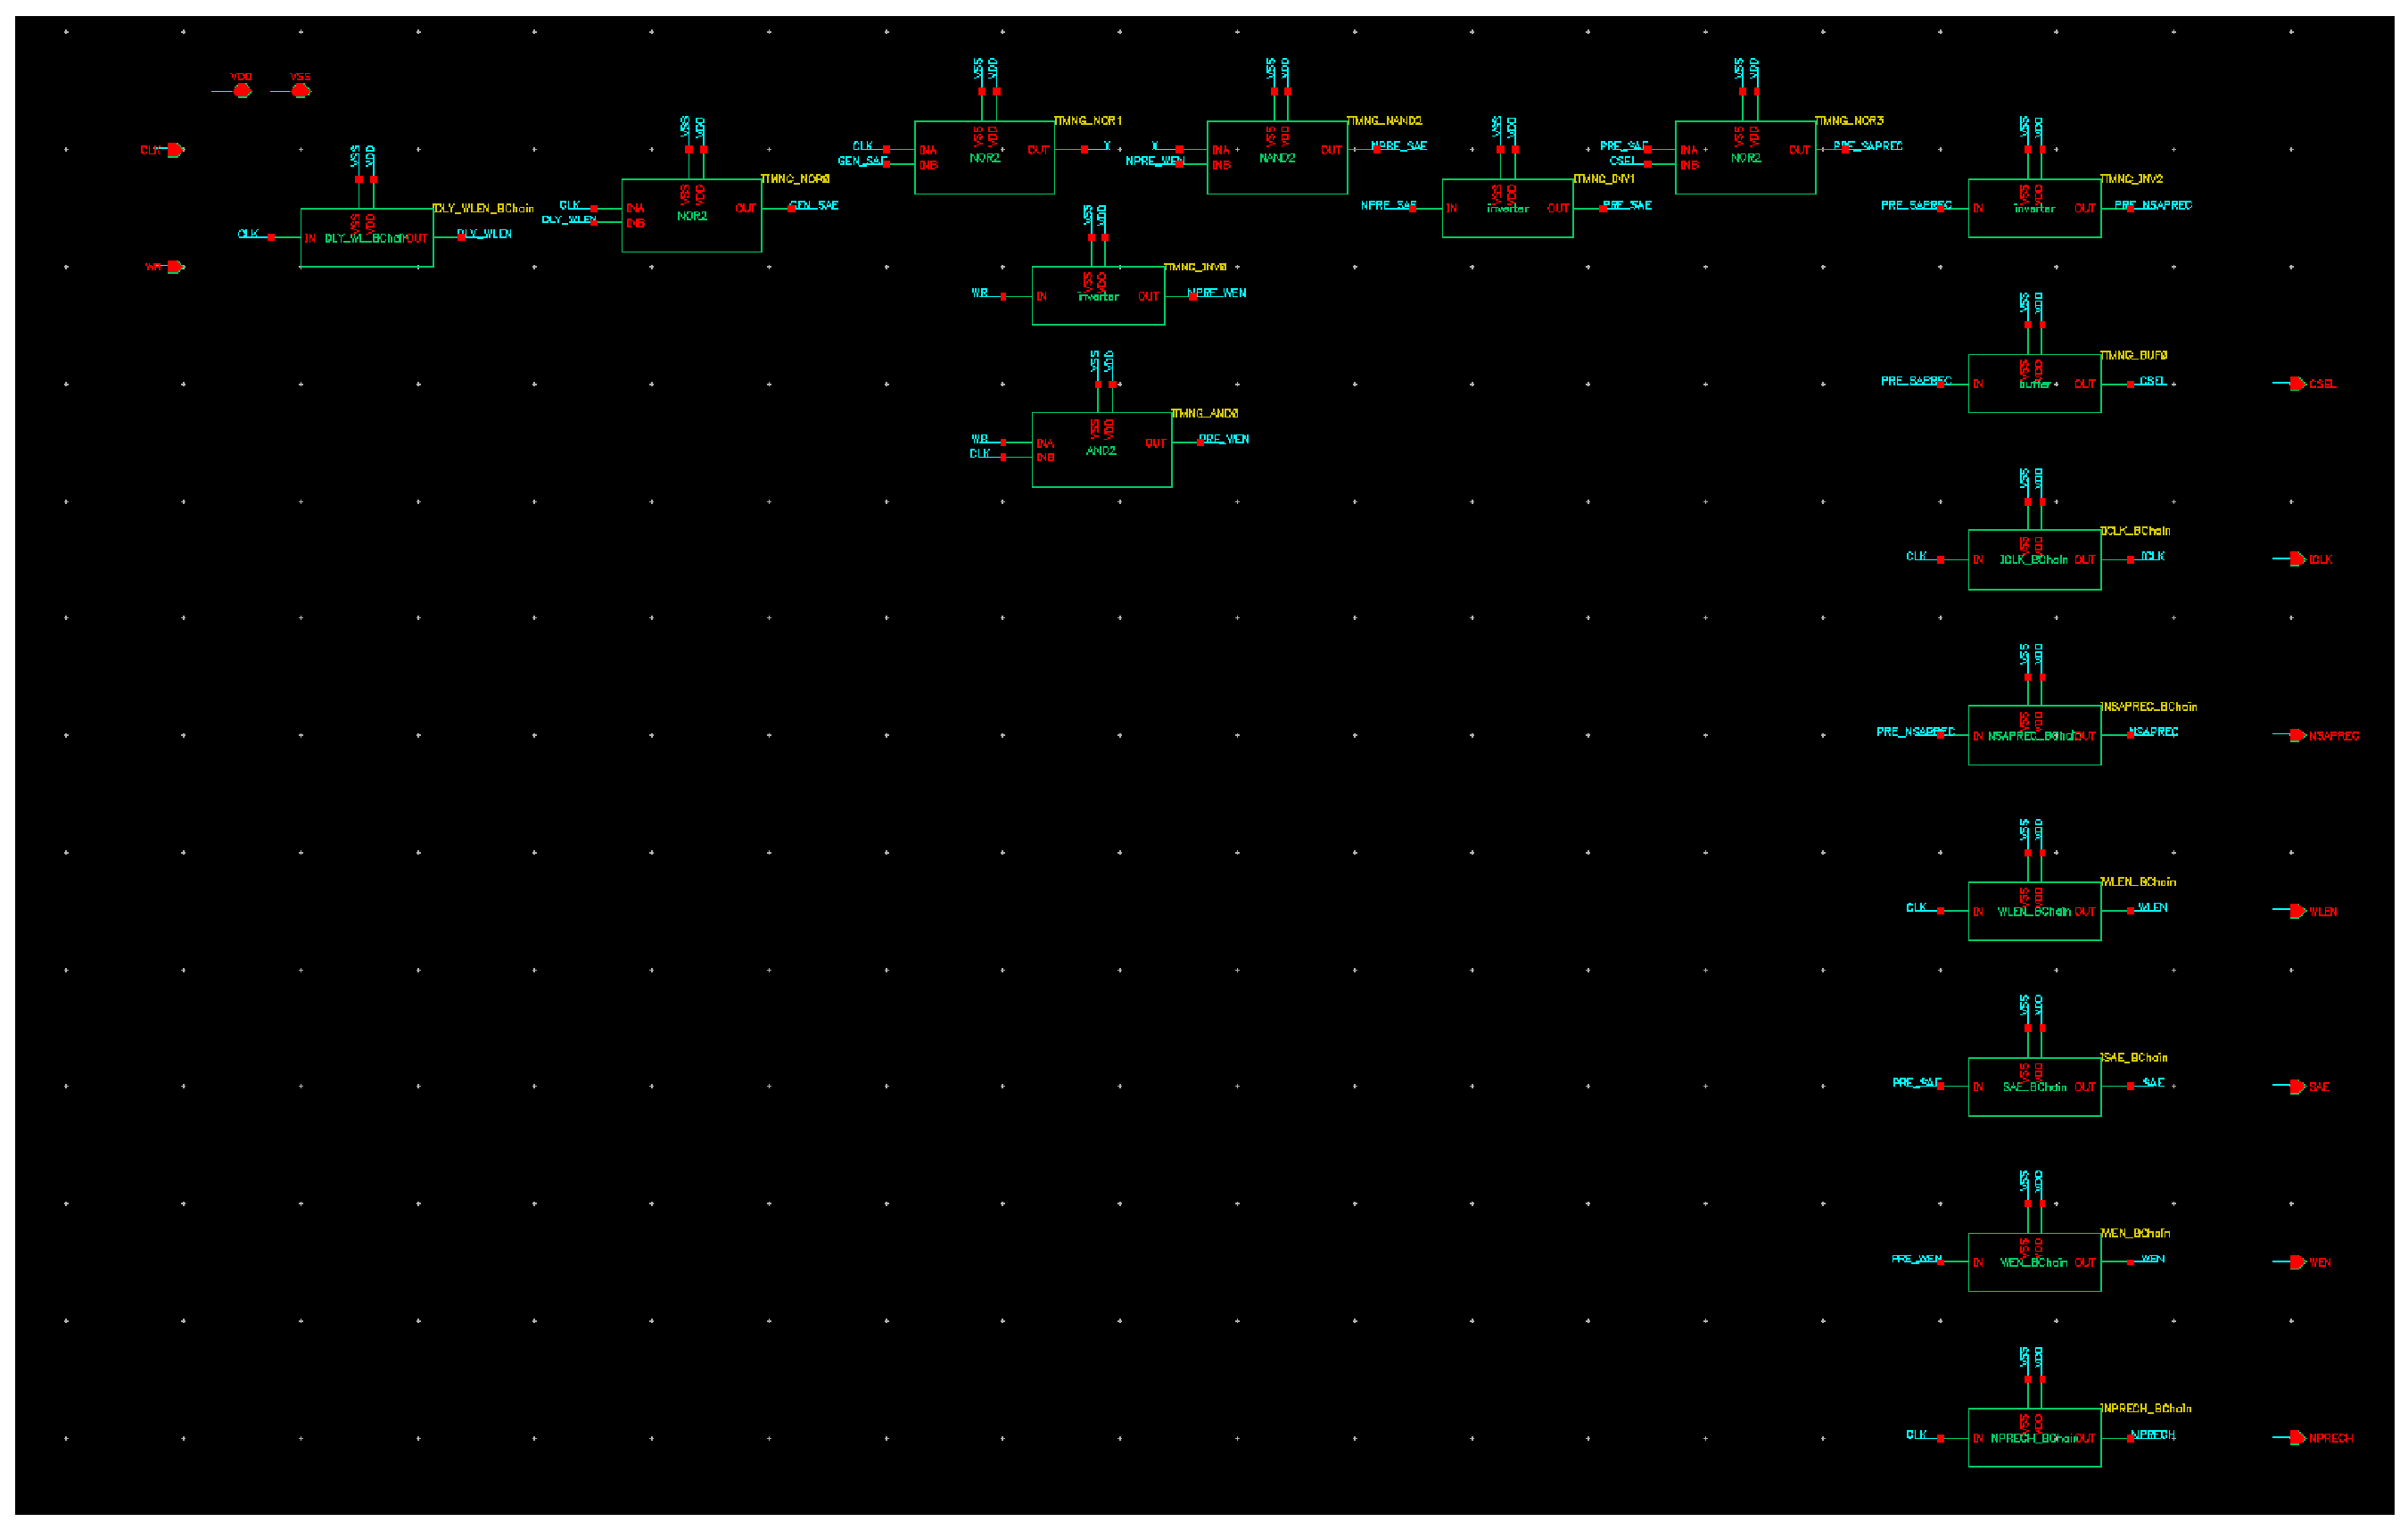
\includegraphics[scale=0.3]{Timing}
\vspace{-5pt}
  \caption{Timing block.}
  \label{fig:tmgblk}
\vspace{-5pt}
\end{figure}

The control signals (listed below), generated for the read and write operations are shown in Figure~\ref{fig:ctrl}. 
\begin{itemize}
\setlength{\itemsep}{0cm}
\setlength{\parskip}{0cm}
\item WEN - Enable for the tri-states in the IO.
\item NPRECH/PCH - BL precharge and equalize transistor control in the CD.
\item NSAPREC/SAPREC - SA precharge control in the SA .
\item CS/CSEL\_i, NCS/CSELB\_i - Column mux transmission gate controls in the CD.
\item SAE - SA enable in the SA.
\item ICLK/OCLK/CLK - CLK signal for different FFs.
\end{itemize}

\begin{figure}[htb]
\centering
\subfigure[]{
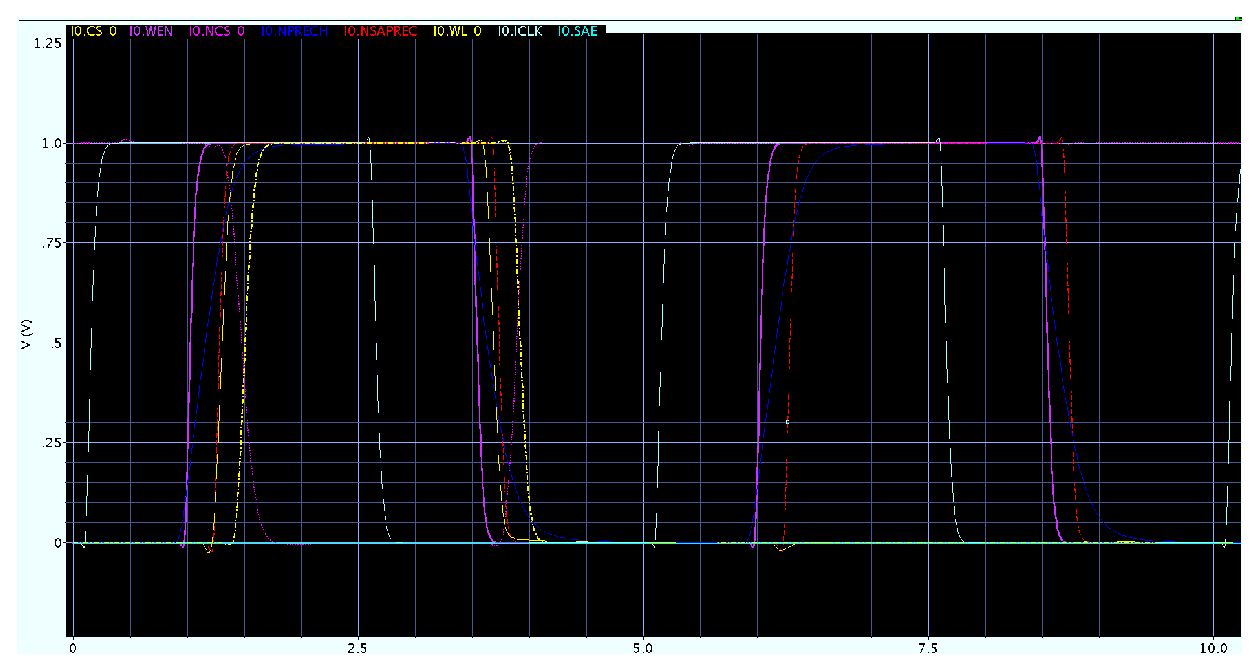
\includegraphics[scale=0.4]{WriteCtrl.eps}
\label{fig:wrt}
}
\subfigure[]{
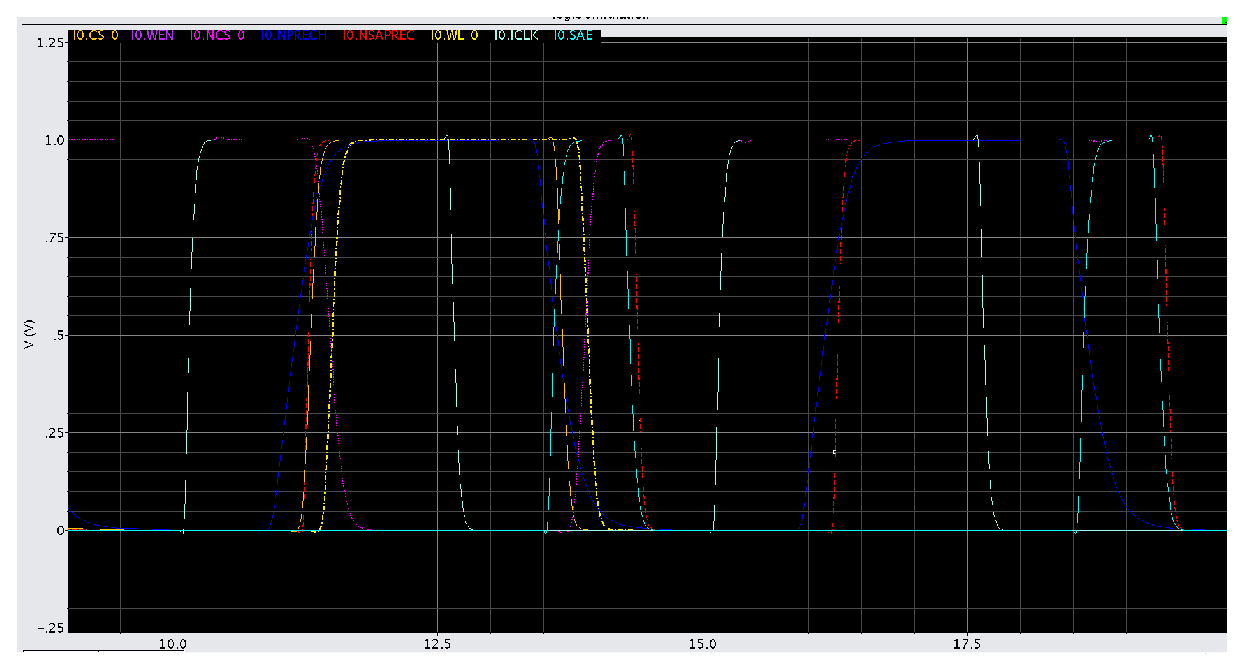
\includegraphics[scale=0.4]{ReadCtrl.eps}
\label{fig:rd}
}
\caption{Timing diagrams showing the control signals for (a) write (b) read}
\label{fig:ctrl}
\end{figure}

The control signals are generated from a clock input to the SRAM, using delay elements. During a write, the control signals (WEN, NPRECH, NSAPREC, CS and NCS) are of the same width and are pulsed some delay after the rising clock edge to allow the address and data inputs to be latched, and to allow the pre-decode and column-decode to finish. The SAE remains low throughout the write cycle. To avoid timing races and to ensure correct functionality, the edges of the pulses should be in the following order (Figure~\ref{fig:wrt}), with an upward arrow indicating a rising edge, and a downward one indicating a falling edge --- WEN$\uparrow$ - NPRECH$\uparrow$ - NSAPREC$\uparrow$ - CS$\uparrow$ - NCS$\downarrow$ - WL$\uparrow$ - WEN$\downarrow$ - NPRECH$\downarrow$ - CS$\downarrow$ - NSAPREC$\downarrow$ - NCS$\uparrow$ - WL$\downarrow$.

During a read, NSAPREC and SAE are not of the same width as the remaining control signals. To ensure that the precharge of the SA inputs is turned off both during the BL differential development, and the SA resolution, the NSAPREC pulse encompasses both these phases. The SAE goes high (e.g. the SA is enabled) towards the end of the WL pulse. The WEN signal remains low throughout the read cycle. The pulse edge order for read is --- NPRECH$\uparrow$ - NSAPREC$\uparrow$ - CS$\uparrow$ - NCS$\downarrow$ - WL$\uparrow$ - SAE$\uparrow$ - CS$\downarrow$ - NCS$\uparrow$ - NPRECH$\downarrow$ - WL$\downarrow$ - SAE$\downarrow$ - NSAPREC$\downarrow$ - ICLK$\uparrow$.

The generation of the control signals can be done using the same logic for any technology. What varies from one technology to another are the characteristics of the buffer chains in the delay elements and the final control signal drivers (e.g. the number of stages, fanout). ViPro can be used to optimize these parameters to ensure proper generation of the control signals in any technology. Section~\ref{sec:opt} discusses the timing optimization in more detail.

\section{Energy and Delay Calculation}
\label{calc}

The devices in each peripheral circuit are parametrized and TASE simulations can determine the E, D characteristics of these circuits across a range of parameters. Both read and write operations can be broken down into two paths --- the circuits between the address and the final WL to the bitcell (Figure~\ref{fig:tmg}), and those driving or receiving the data from the BL(Figure~\ref{fig:col}). Energy and delay or min. cycle time for the SRAM are calculated from the component Es and Ds along these paths, using the following model.
  
\begin{figure}[htb]
  \centering
  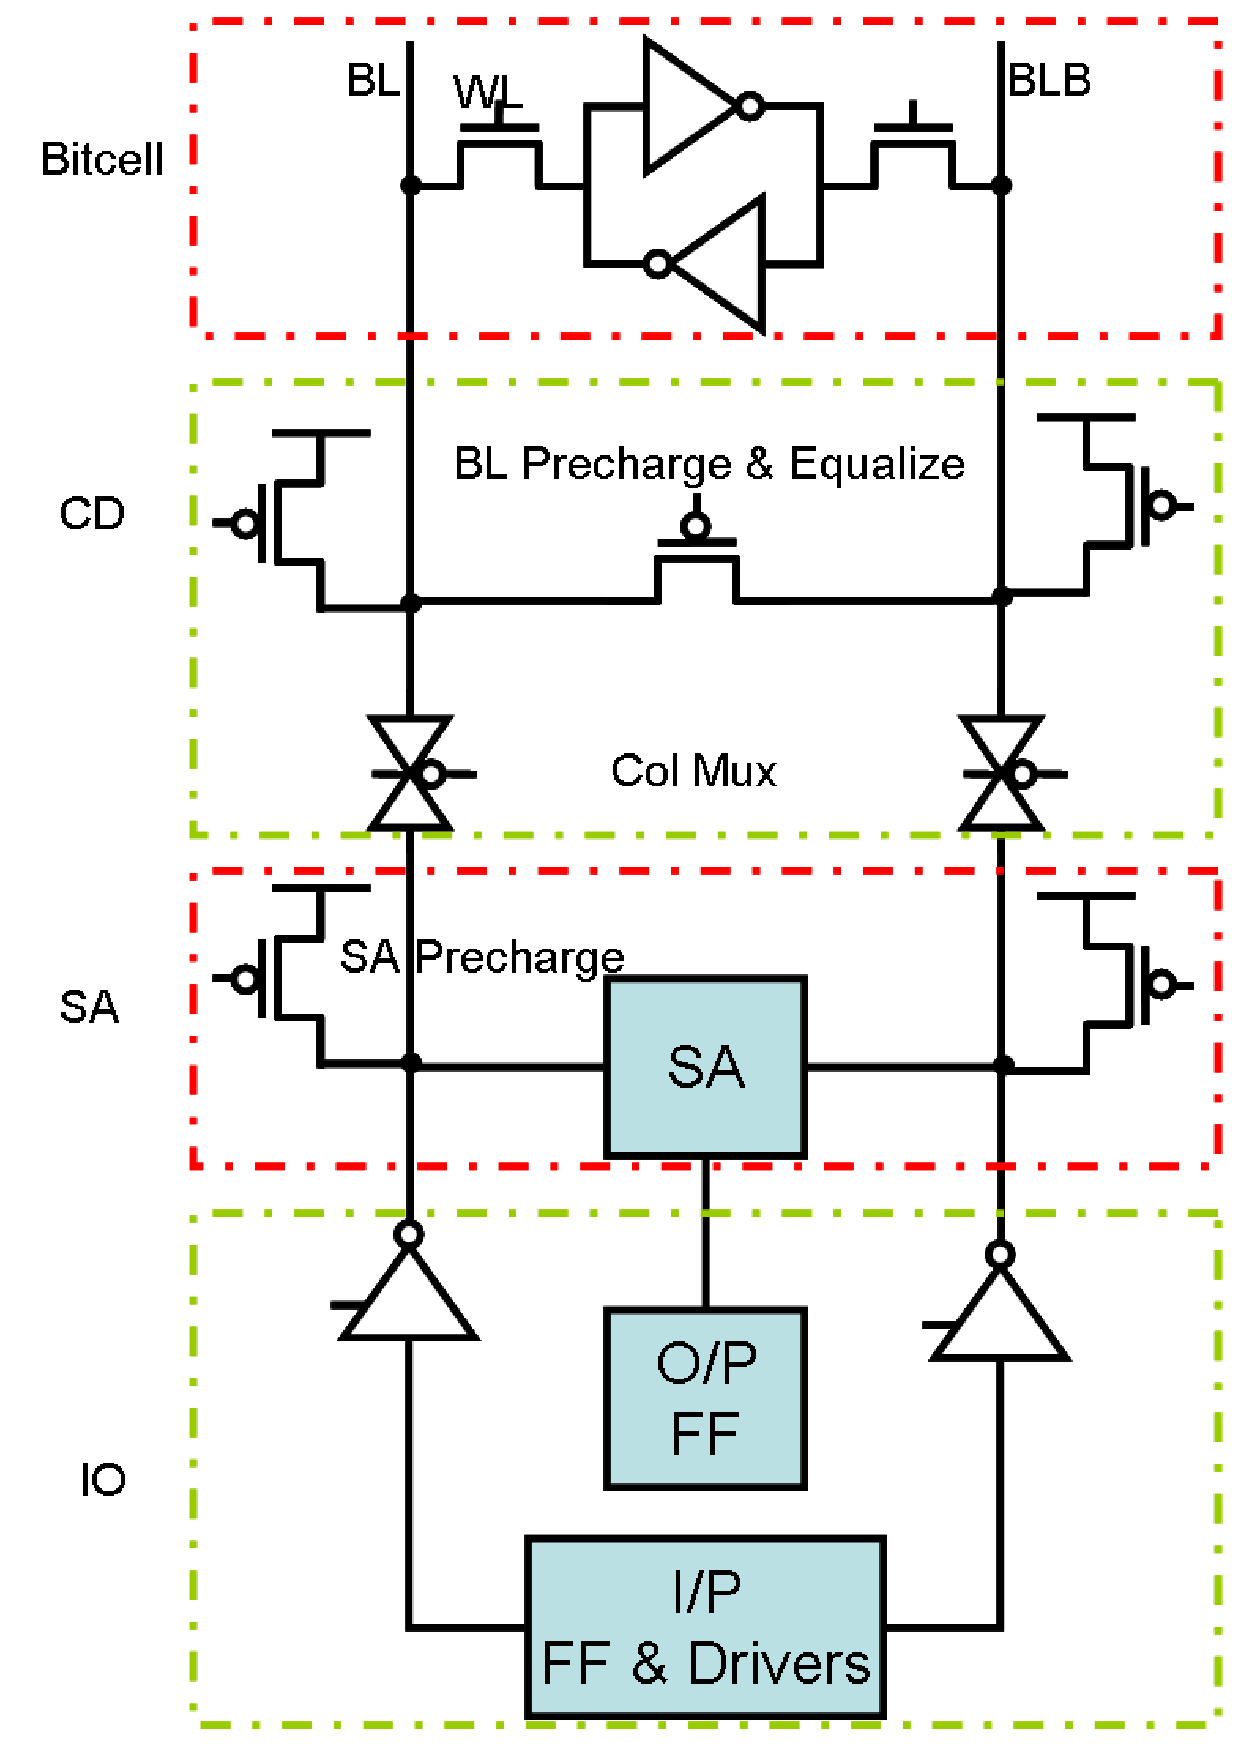
\includegraphics[scale=0.35]{Vipro_col}
\vspace{-5pt}
  \caption{A single column and its associated circuitry}
  \label{fig:col}
\vspace{-5pt}
\end{figure}

\subsection{Write}
The minimum cycle time is determined by the critical path delay of the SRAM during a write. The write operation can be broken down roughly into three stages (Figure~\ref{fig:wrtstg}). The first (s1) is the predecode/col-decode and address/data latch stage. The second (s2) is the WL enabled stage where the cell flips. The final (s3) stage is the precharge stage where the BLs are precharged back to prepare for the next access cycle. s3 can occur in parallel with s1 of the next cycle. In sum, the write operation consists of the following actions. 
\begin{enumerate}
\setlength{\itemsep}{0cm}
\setlength{\parskip}{0cm}
\item Input data latching in IO (`io')
\item Row pre-decode (`rowpre')
\item Column decode (`coldec')
\item WL enable (`wld')
\item Bitcell node flip (`bcwr')
\item Precharge BL/BLB (`cdch')
\item Precharge RDWR/NRDWR (`sach')
\end{enumerate}

\begin{figure}[htb]
  \centering
  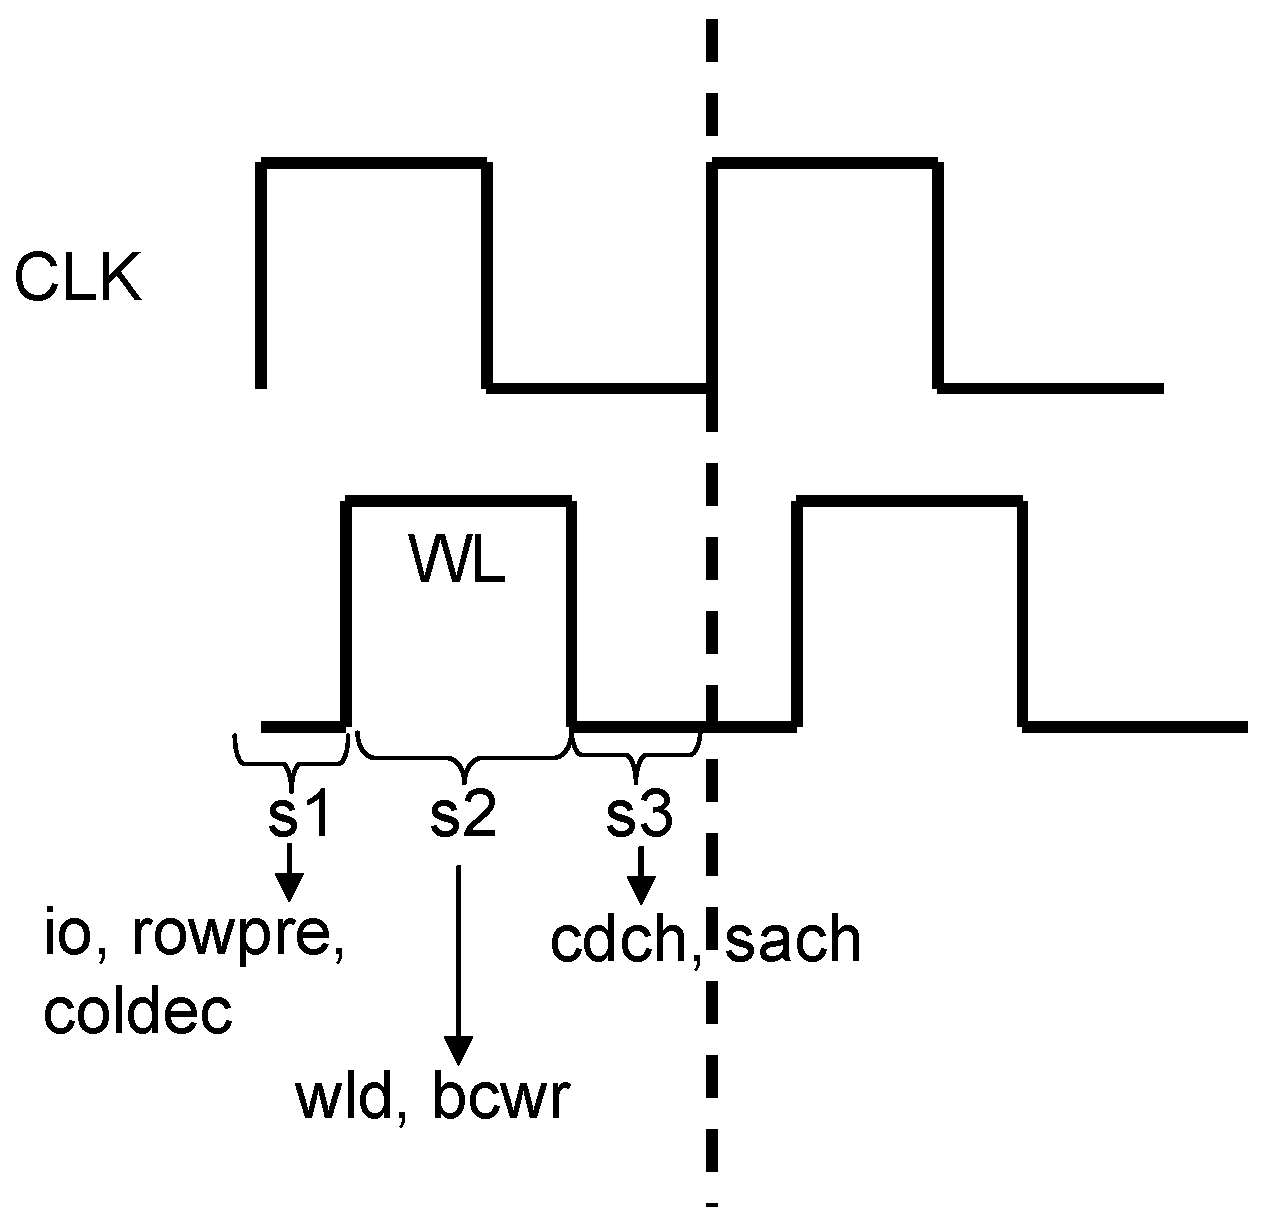
\includegraphics[scale=0.3]{wrtStg}
\vspace{-5pt}
  \caption{Stages of the write operation}
  \label{fig:wrtstg}
\vspace{-5pt}
\end{figure}

The minimum cycle time for write (T$_\text{MIN-W}$) can be determined as:
\begin{equation}\label{tminw}
\displaystyle  T_{MIN-W}=max(io,rowpre,colpre,cdch,sach) + wld + bcwr
\end{equation} 

If s1 is the bottleneck, s3 of the previous stage can occur in parallel. Thus, a separate pre-charge stage is not required for the write operation and there are effectively only two stages. In this case, the minimum write cycle reduces to 
\begin{equation}\label{tminw}
\displaystyle  T_{MIN-W}=max(io,rowpre,colpre) + wld + bcwr
\end{equation} 

If s3 is the bottleneck, some extra time (s3) is required after s2. The total time available for s3 and the s1 of the next stage should be sufficient to precharge the column. In this case, the minimum write cycle reduces to 
\begin{equation}\label{tminw}
\displaystyle  T_{MIN-W}=max(cdch,sach) + wld + bcwr
\end{equation} 

The energy per access (read or write) is calculated by summing up the energy contributed by each component. The energy is calculated in the following way. First, the average power is measured using-

\begin{verbatim}  
average(getData("<component>:pwr"))
\end{verbatim}

This is the average power measured over the entire simulation time, and does not necessarily correspond to the average power over the actual cycle time. However, the measured energy, which is average power$\times$simulation time will nearly be equal to the actual energy expended in the cycle, except for the leakage energy, which for the peripheral components can be considered to be negligible compared to the switching energy. Thus, we measure the average power and get the energy first by multiplying the simulation time. The top-level SRAM energy is then the sum of the energies of the individual componenets. The top-level SRAM power can now be estimated by multiplying this number with the frequency of operation.

We now briefly discuss the energy calculation during the write operation.
\subsubsection{Bitcell}
The energy dissipated in the bitcell during the write is due to the switching of the storage nodes. As can be seen in Figure~\ref{fig:write_bc}, when the BLs and storage nodes are at opposite values, there is energy dissipated in the bitcell, through the on access transistors. Once the flip nears completion and the V$_\text{DS}$ reduces for the access transistors, the energy goes to zero. The total bitcell write energy can be calculated by multiplying with the number of cells being written, i.e. the word size.

There is also energy dissipated in the half-selected bitcells on the same row, which do a dummy read. This component of the bitcell energy during write can be estimated by multiplying the read energy of the bitcell with the number of unselected columns (i.e. half-selected cell), which is equal to the number of columns minus the word-size.

\begin{figure}[htb]
  \centering
  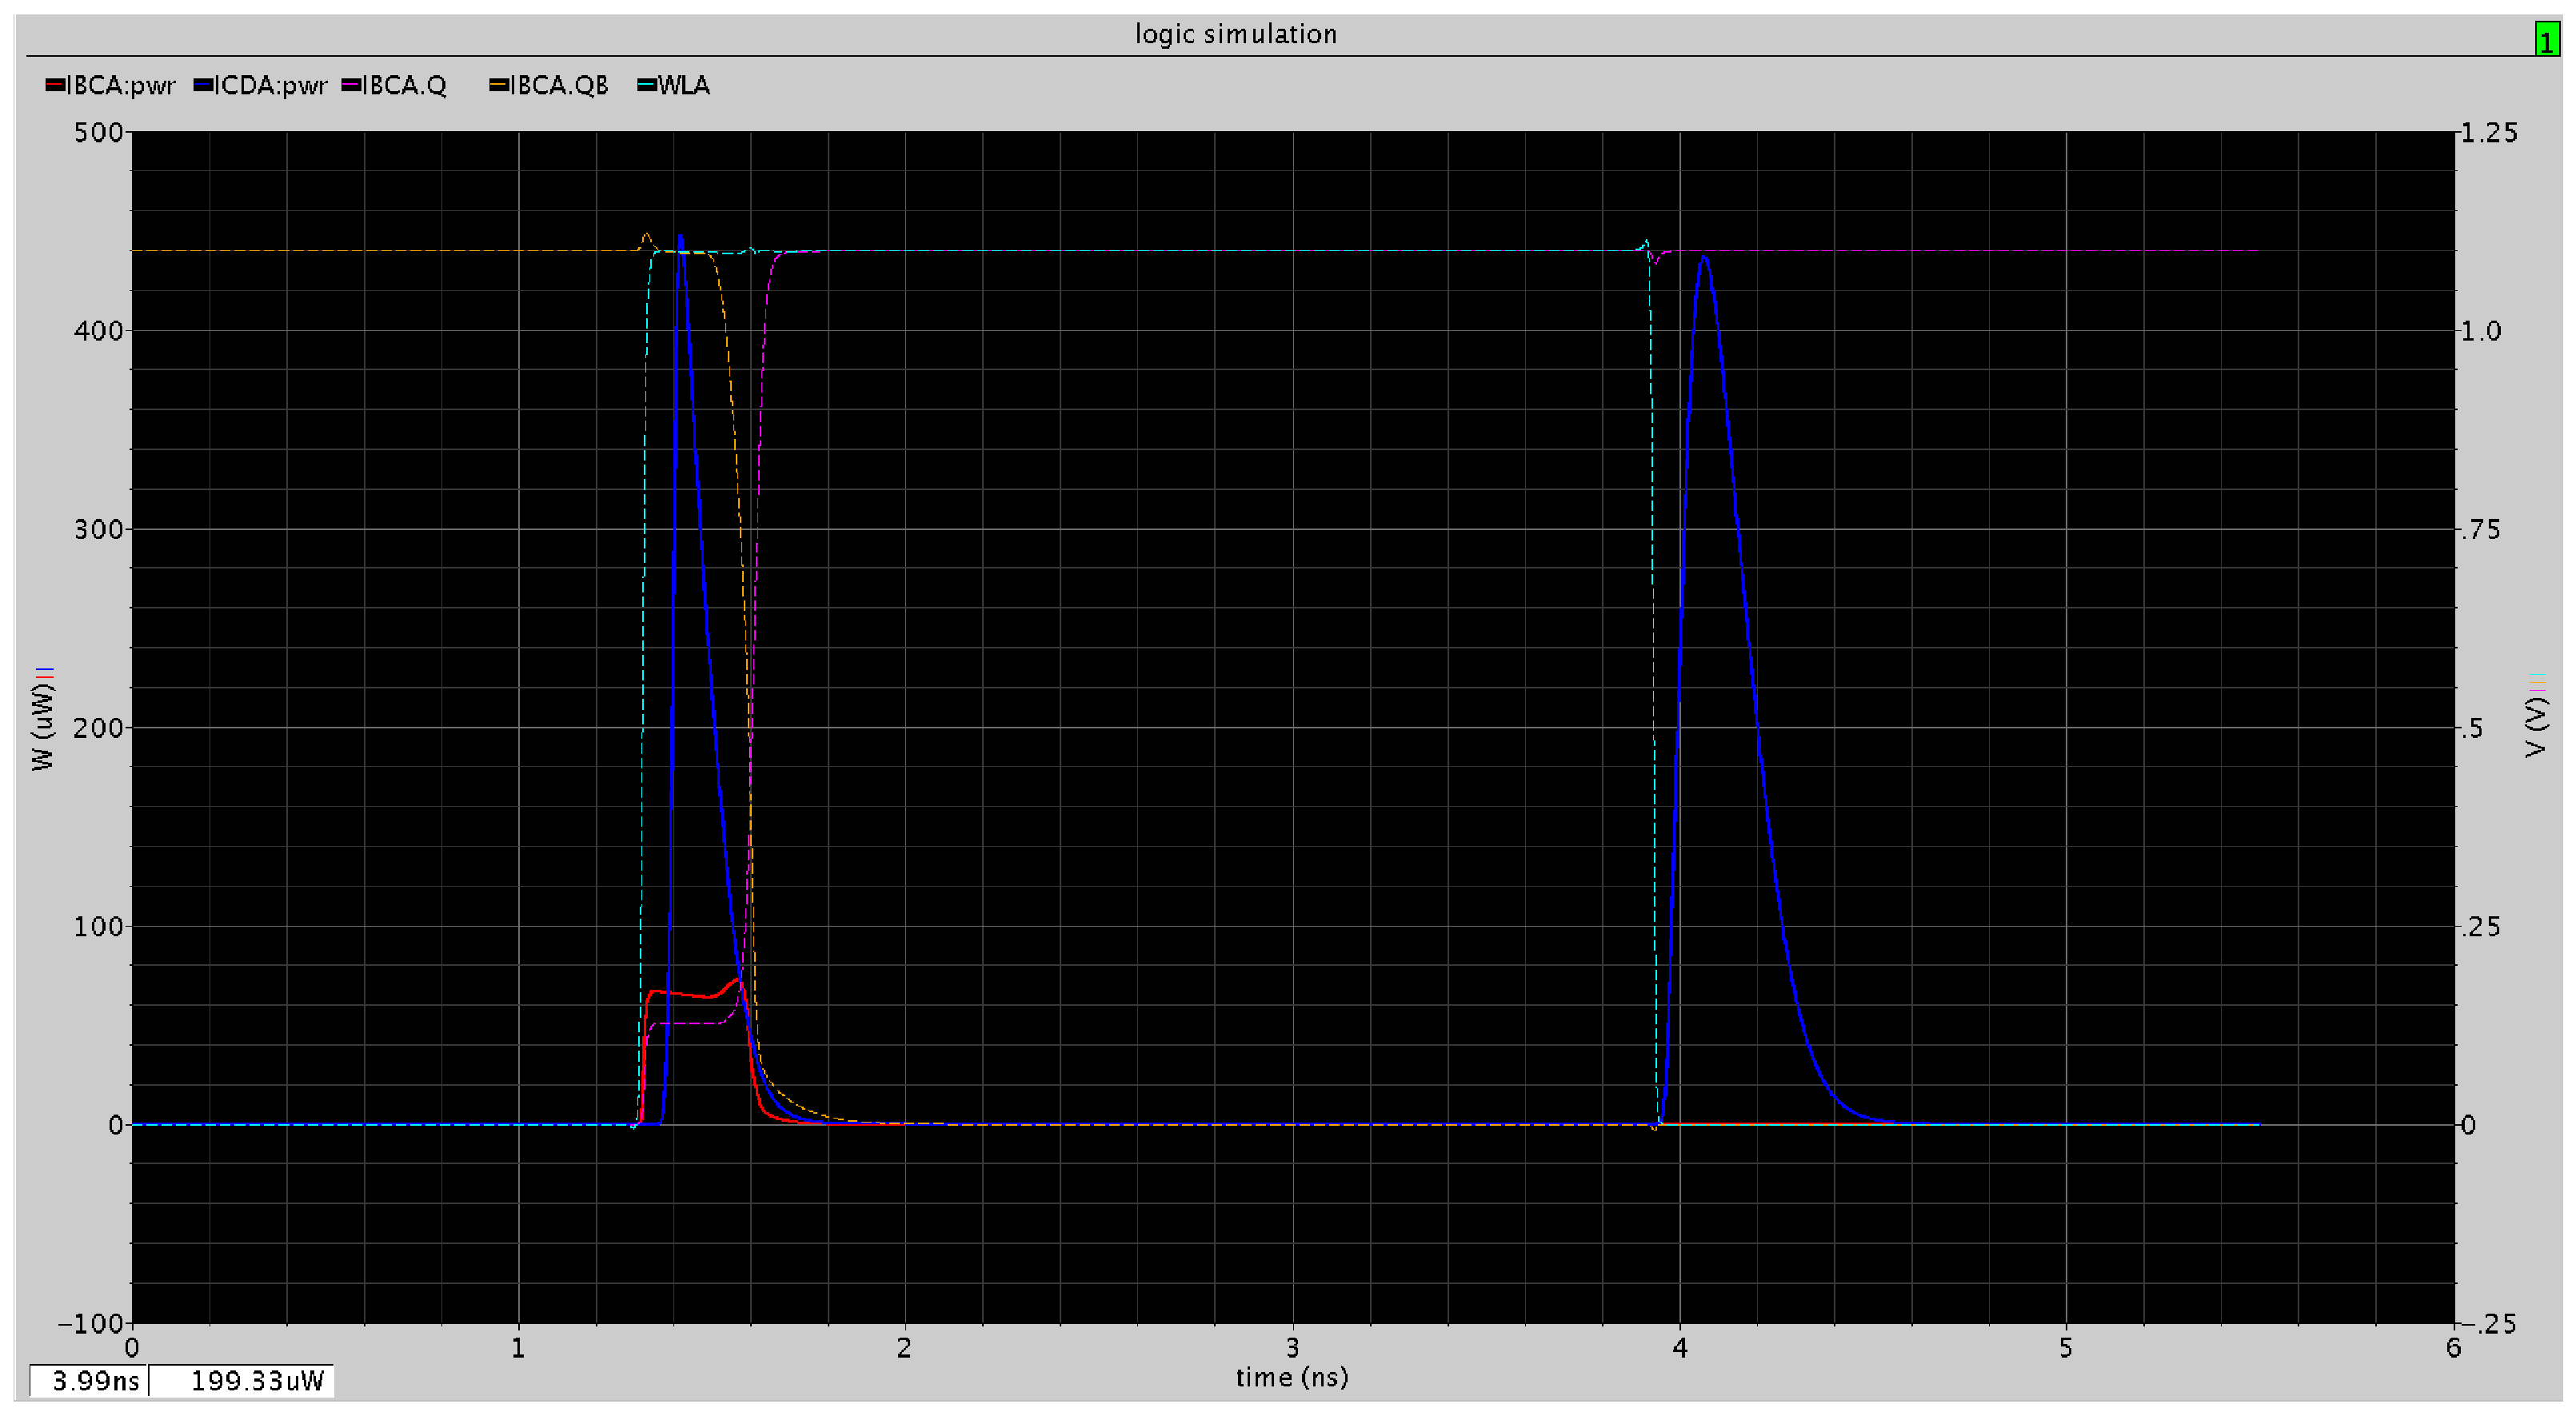
\includegraphics[scale=0.25]{BC_Write_ptm65}
\vspace{-5pt}
  \caption{Signals and power waveforms for bitcell power during write.}
  \label{fig:write_bc}
\vspace{-5pt}
\end{figure}

\subsubsection{CD}
The CD dissipates power at two points during the write cycle, as seen in Figure~\ref{fig:write_cd}. The first occurs when the column mux trasistors turn on. Energy is dissipated through the transmission gate on the side where the BL is discharging through the PD in the write driver. The BLs are assumed precharged in the sim, so there is no power dissipated by the precharge FET on this side when the WL goes high. The second part of the power dissipation is due to the precharge through the PMOS after the WL has gone low. At this point, the col-mux FETS are off, so the PMOS precharge accounts for the entire power at this point. The total power dissipated in the CD by the accessed columns can be determined by multiplying with the word size as with the bitcell power described above.

The unselected columns have only one component of power dissipation during the write, which is the power dissipated to precharge the bitlines which have drooped due to a dummy read. Multiplying the read CD power (described in the next section) with the number of unselected columns gives the total power.

\begin{figure}[htb]
  \centering
  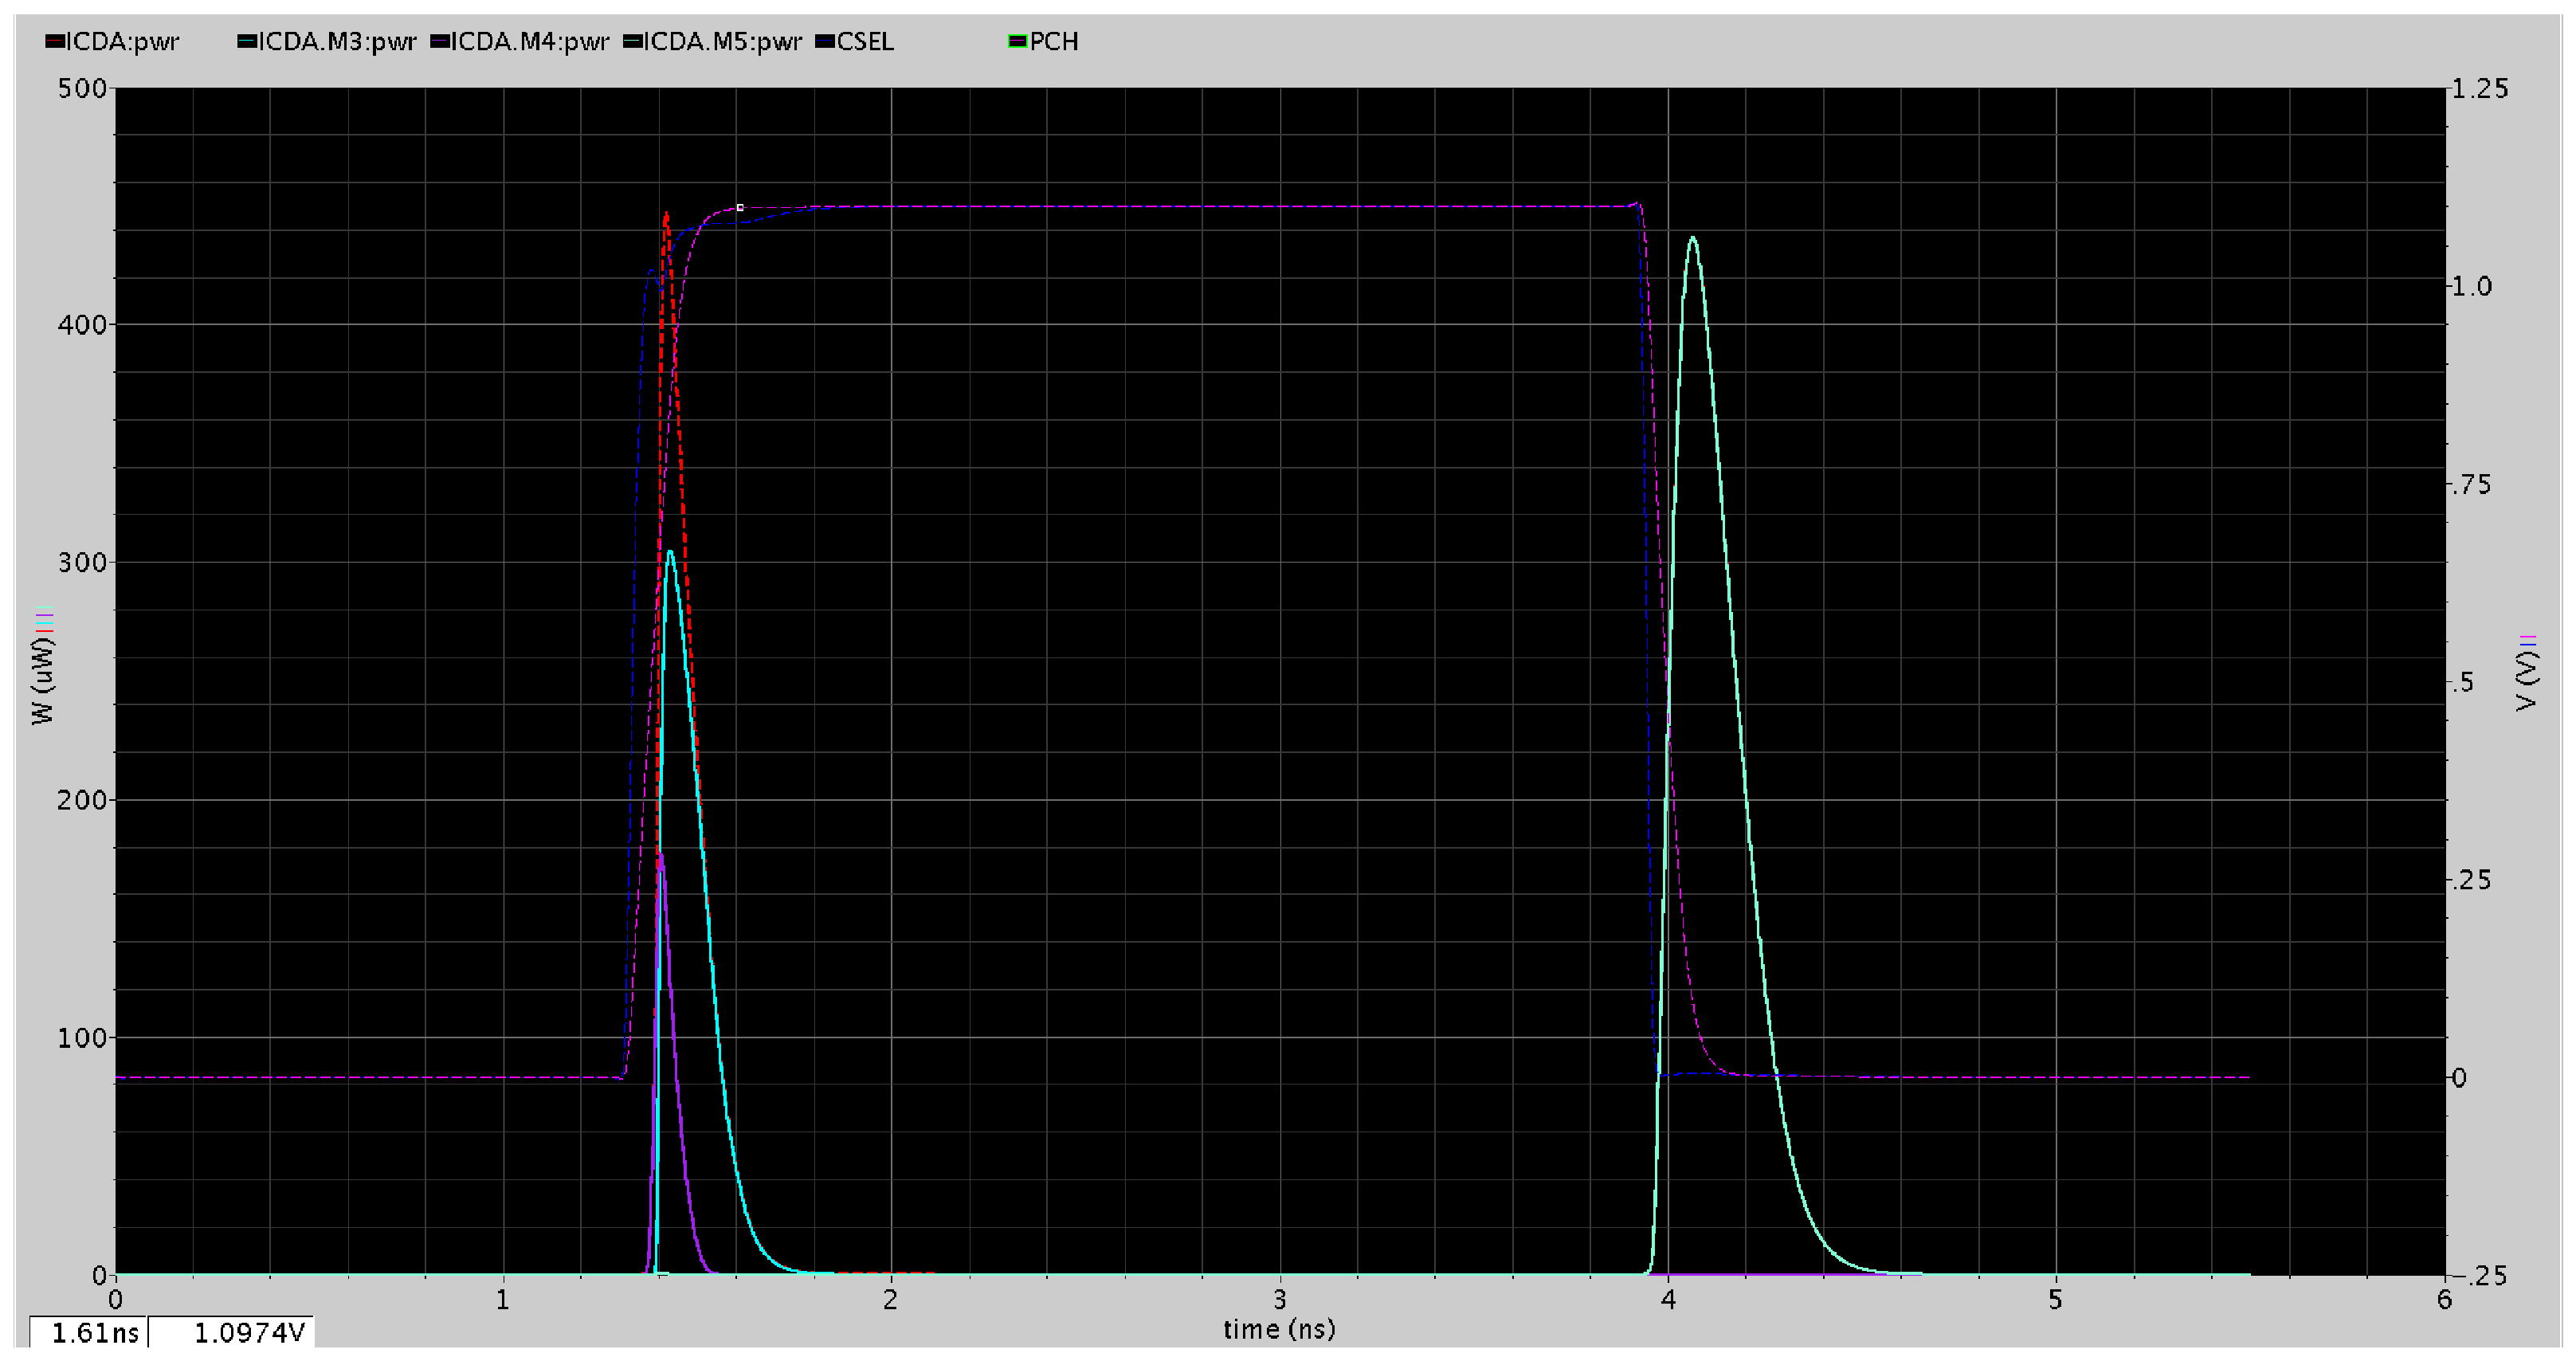
\includegraphics[scale=0.25]{CD_Write_ptm65}
\vspace{-5pt}
  \caption{Signals and power waveforms for CD power during write.}
  \label{fig:write_cd}
\vspace{-5pt}
\end{figure}

\subsubsection{SA}
During the write, since the SA does not sense, the power that is dissipated is due to the pre-charging of one of the NRDWR/RDWR nodes depending on what data was written. Figure~\ref{fig:write_sa} shows the entire power to be due to the precharging of the NRDWR node through the PMOS precharge device. Multiplying the measured power with the word size gives the total power.

\begin{figure}[htb]
  \centering
  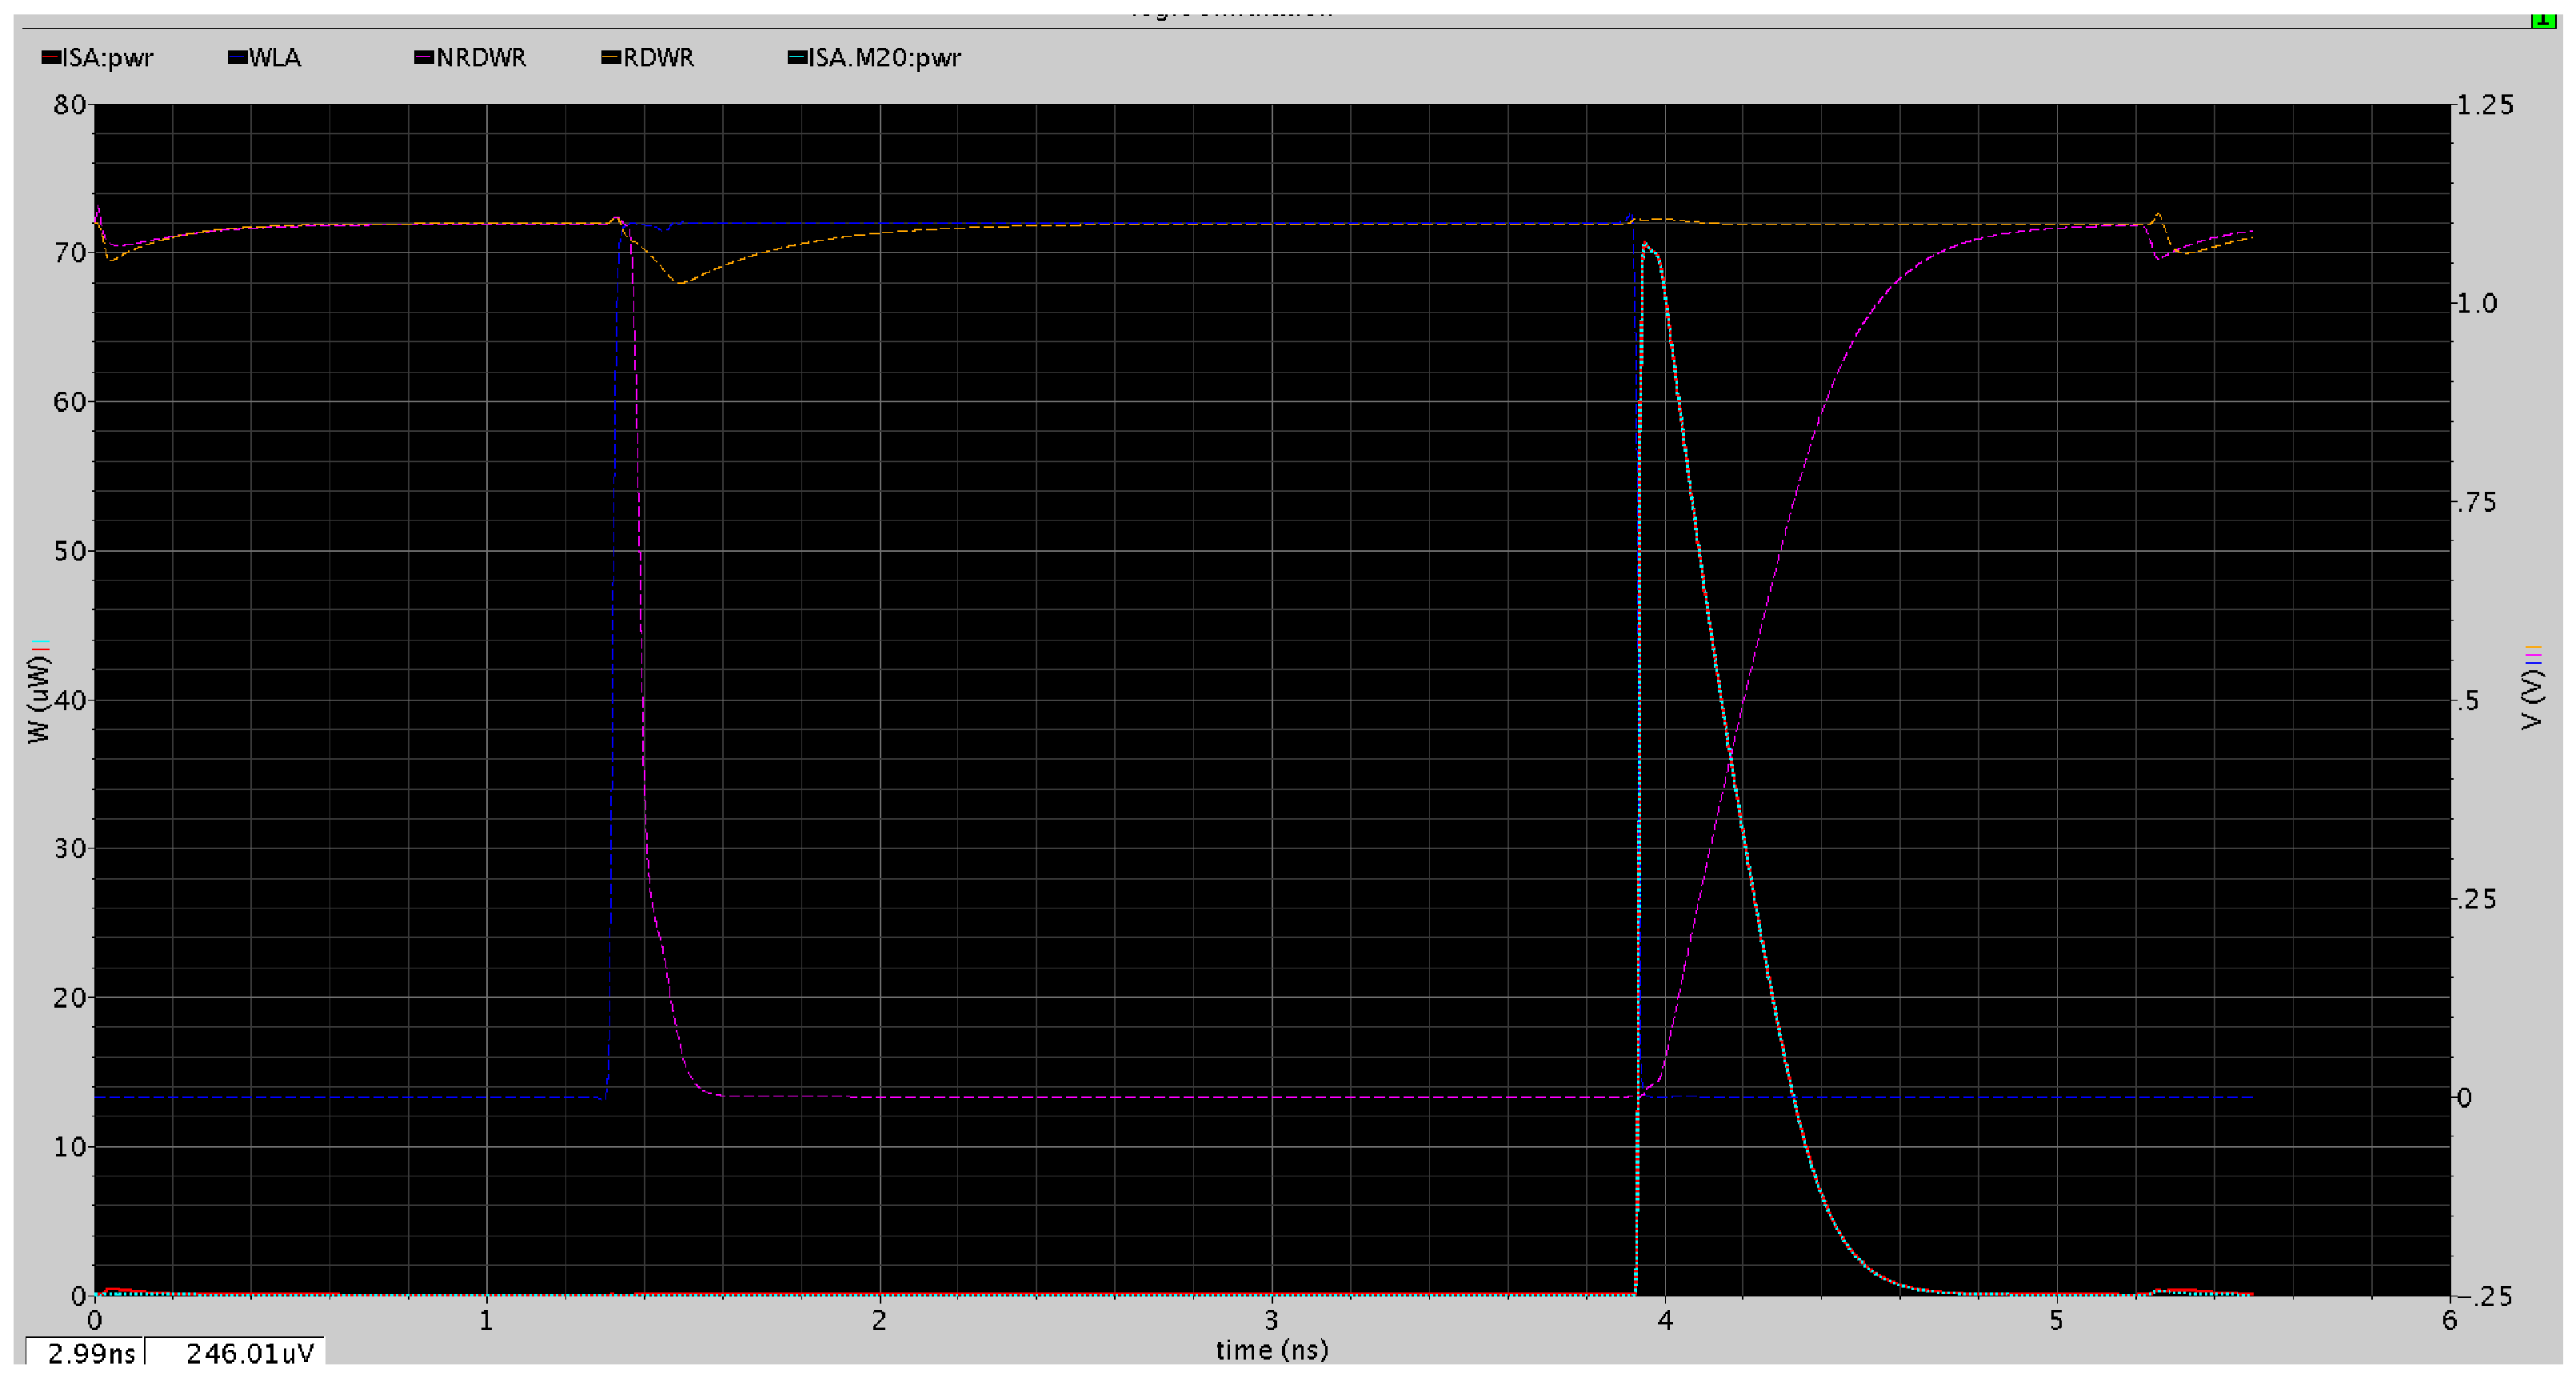
\includegraphics[scale=0.25]{SA_Write_ptm65}
\vspace{-5pt}
  \caption{Signals and power waveforms for SA power during write.}
  \label{fig:write_sa}
\vspace{-5pt}
\end{figure}

\subsubsection{IO}\label{wrtpwr_io}
Figure~\ref{fig:write_io} shows the signals and power waveforms in the IO during a write. There are 4 events that cause power dissipation as can be seen from the figure. First, the rising CLK edge causes both DFFs to consume some power. The Write DFF also consumes power due to latching of the new data value. Consequently, the inverter also flips and contributes to the power at this time. The power consumption of the tri-state inverter driving NRDWR is because one of the PD NFETS turns on when the data gets latched.

Second, when the WEN signal goes high, the tri-state inverters consume power. The RDWR tri-inverter consumes less power since one PD FET turns on while the other turns off, but the PD network of the NRDWR tri-inverter is fully turned on when the WEN signal goes high. So, it dominates the power consumption at this time as one bitline is driven to ground. The other component of power dissipation at this time is due to the switching of the inverters in the WEN buffer.

The third event of power consumption is at the clock falling edge when both DFFs consume power. The final event is when WEN goes low again. At this time the WEN buffer inverters consume power. Also, the first two stages in the write DFF consume power due to the change in the data input at this time.

\begin{figure}[htb]
  \centering
  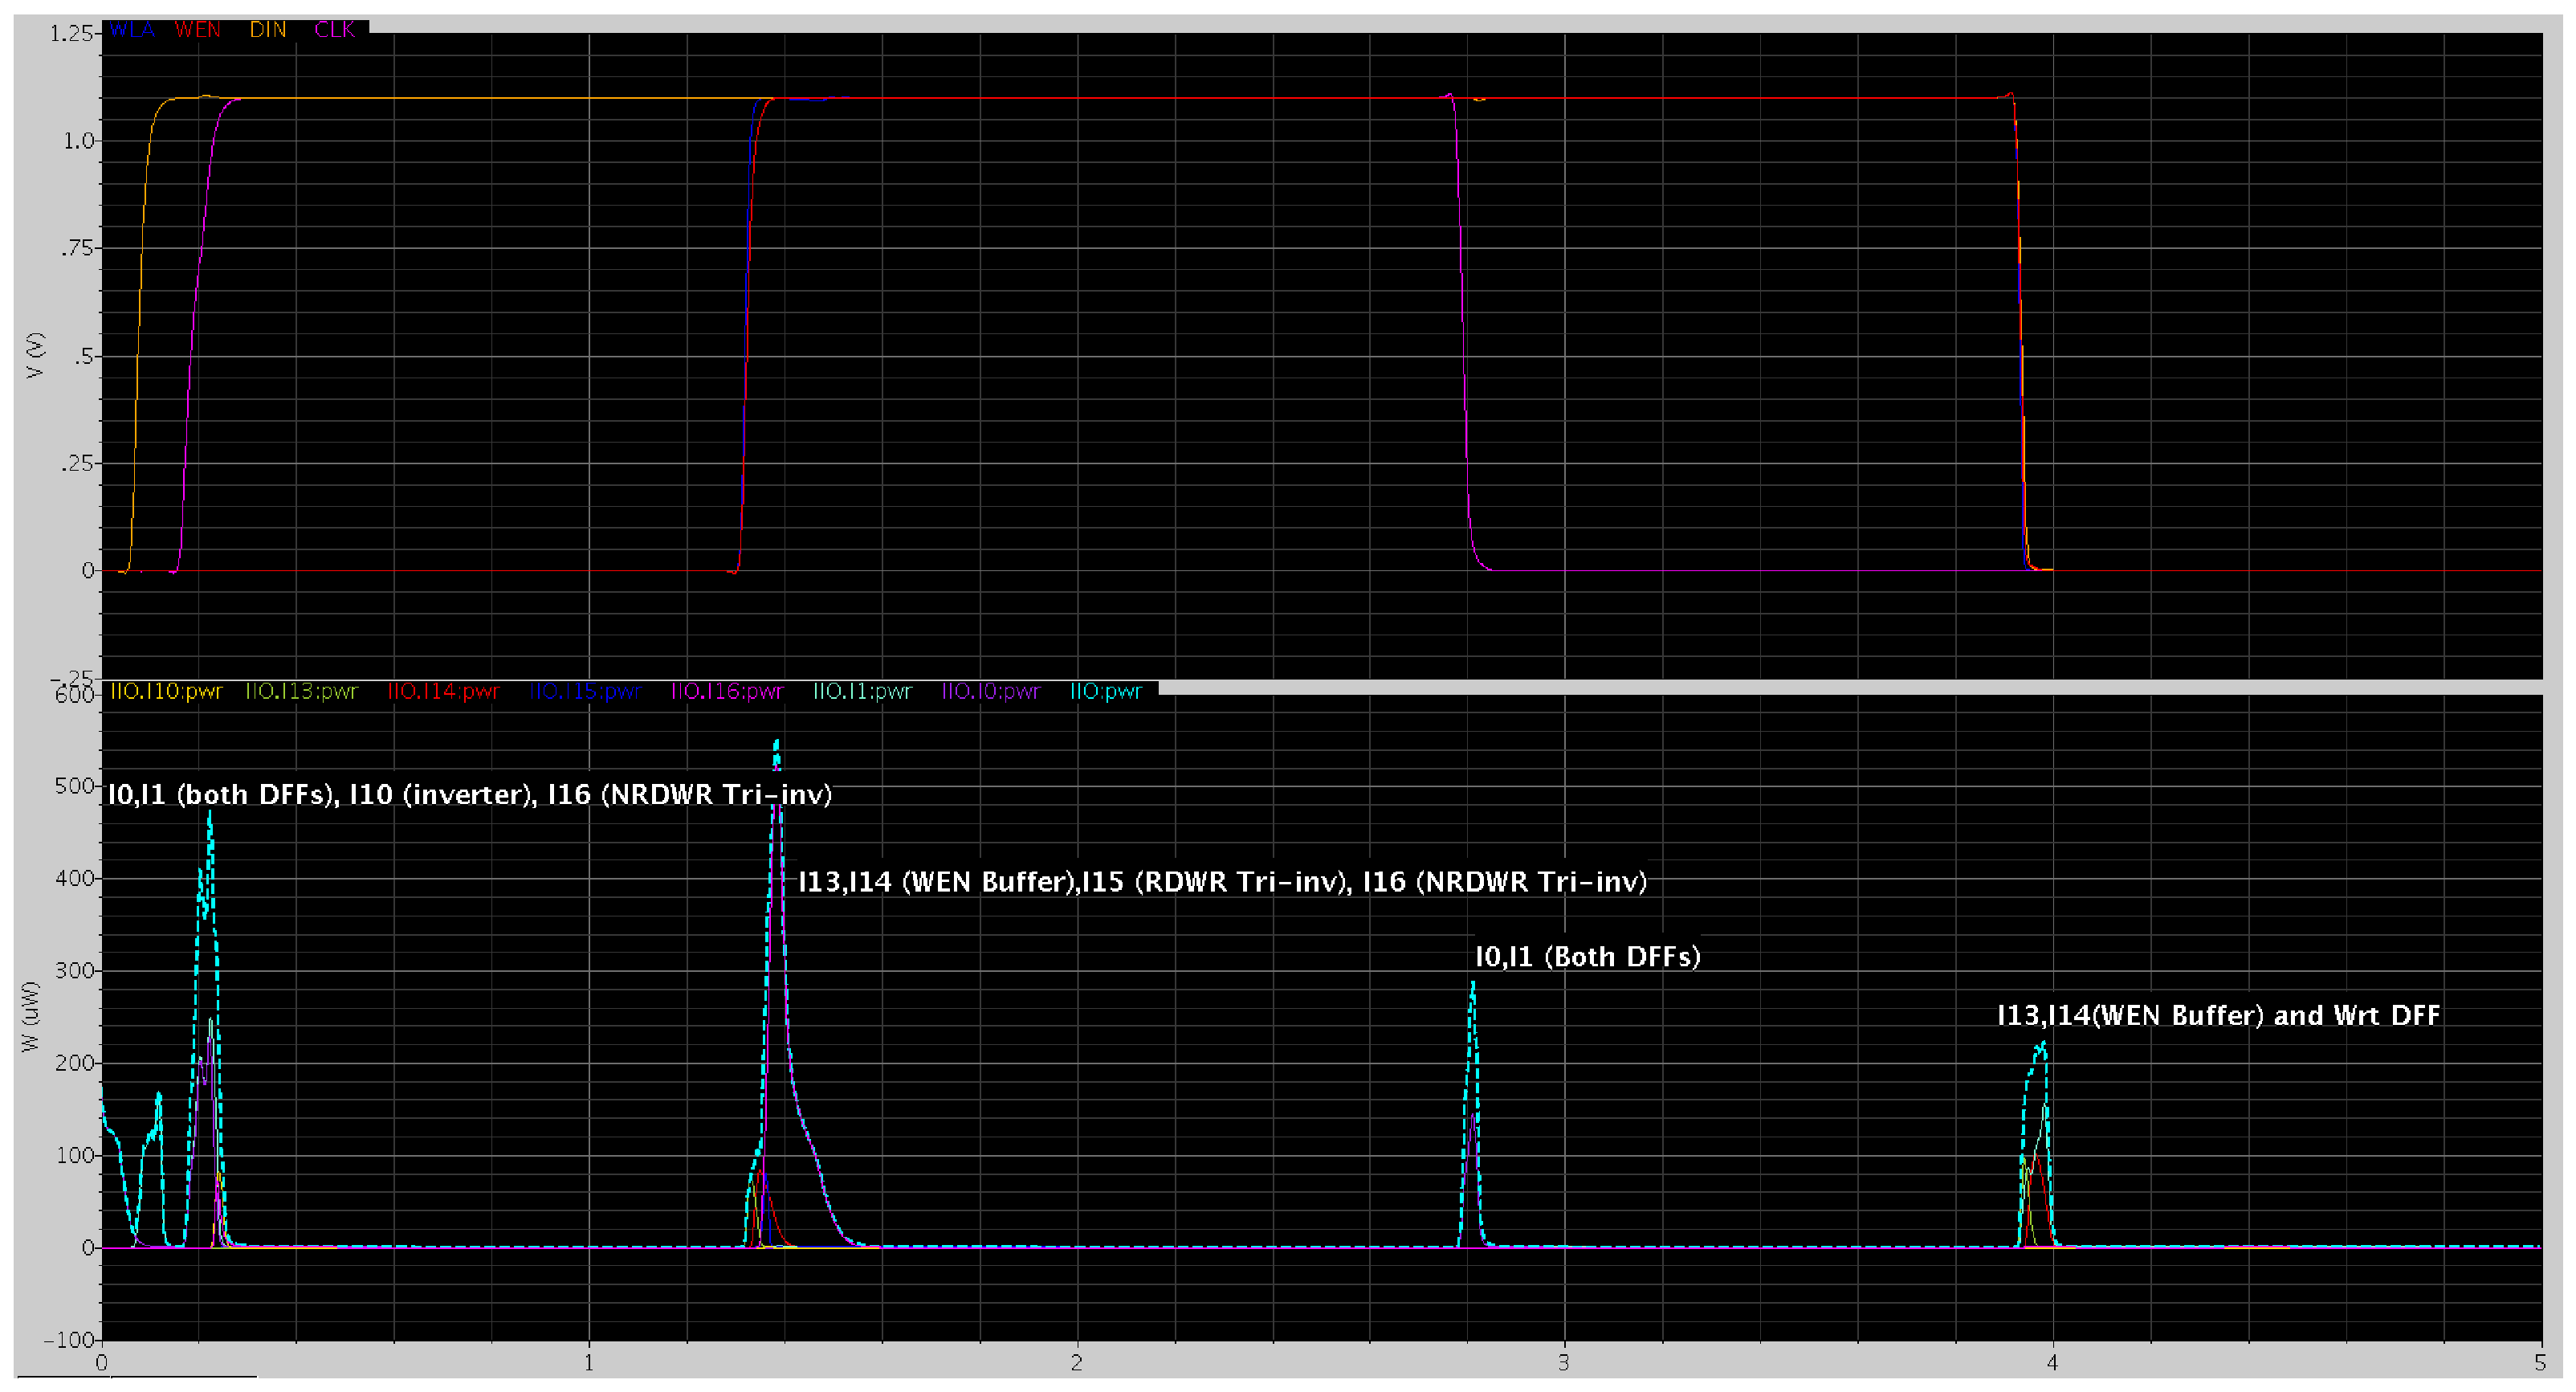
\includegraphics[scale=0.25]{IO_Write_ptm65}
\vspace{-5pt}
  \caption{Signals and power waveforms for IO power during write.}
  \label{fig:write_io}
\vspace{-5pt}
\end{figure}

\subsubsection{Timing}
The average power consumed during write and read is measured. Power is mainly consumed for driving all the control signals horizontally to the bitslice components and vertically to the WL drivers. Since breaking the power down and analyzing it is too complex, we do not describe the timing block power in this document.

\subsubsection{Decoder}
To determine the row decoder and WL driver delays it is sufficient to simulate only the critical path of the decoder. The critical path consists of a predecode phase that drives the vertical predecoded signals to the final decode stage and WL driver that is pitch-matched with each row of the memory. The structure of the critical path varies depending on the number of decoder inputs. We have verified that the power or energy of the critical path is only marginally less (less than 5\%) than that obtained by simulating the whole decoder. So we use the same critical path circuit to determine the energy as well.

The column decoder is a 3 to 8 decoder. The column decoder critical path has a similar gate composition as the 3 to 8 row decoder critical path but for two key differences. One is that there is no intermediate long wire like in the case of the row decoder. The second is the output load being driven by the column decoder, which is composed of the gate caps of the column-mux transmission gates instead of the WL gate capacitances of the bitcells. 

Critical paths for the row and column decoder are shown in Figure~\ref{fig:decCrit}. For the row decoder, buffer chains are tagged on to the end of the predecode and WL driver stages to be able to drive the large capacitances on their outputs. The number of buffer stages in each part of the row decoder is used as a knob in the decoder E-D characterization, as described in ~\ref{subsubsec:decoder}. For the column decoder, the "predecode" is the full 3 to 8 decoder. The second part consists of simply a NAND/AND to combine the decoded output with the column enable signal. The output of this goes to the gates of the column mux transmission gates. The structure of the column decoder critical path is similar to that of a 3 to 8 row decoder with both consisting of only a single NAND/AND in the second (WL Driver) part.

\begin{figure}[htb]
  \centering
  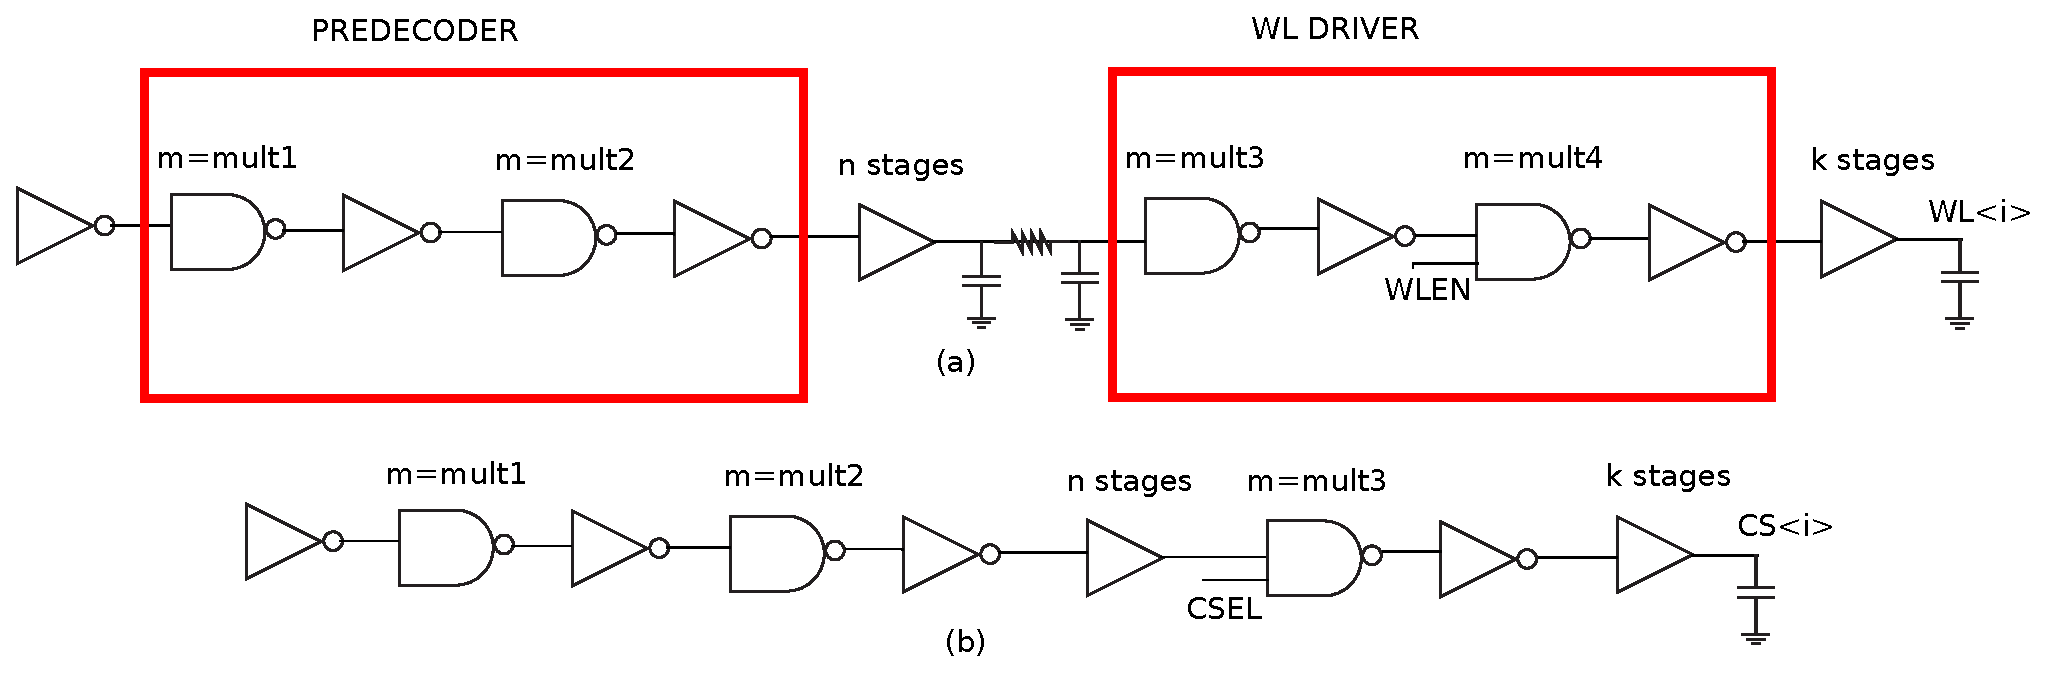
\includegraphics[scale=0.4]{decoder}
\vspace{-5pt}
  \caption{Critical paths for (a)row and (b)column decoder.}
  \label{fig:decCrit}
\vspace{-5pt}
\end{figure}

Figure~\ref{fig:decPower1} shows the power waveforms for various gates in the critical path of the decoder. As Figure~\ref{fig:decPower2} shows, most of the power is dissipated in the final buffer stages of the predecode and the WL driver sections of the decoder since they are big gates driving large load capacitances.
\begin{figure}[htb]
  \centering
  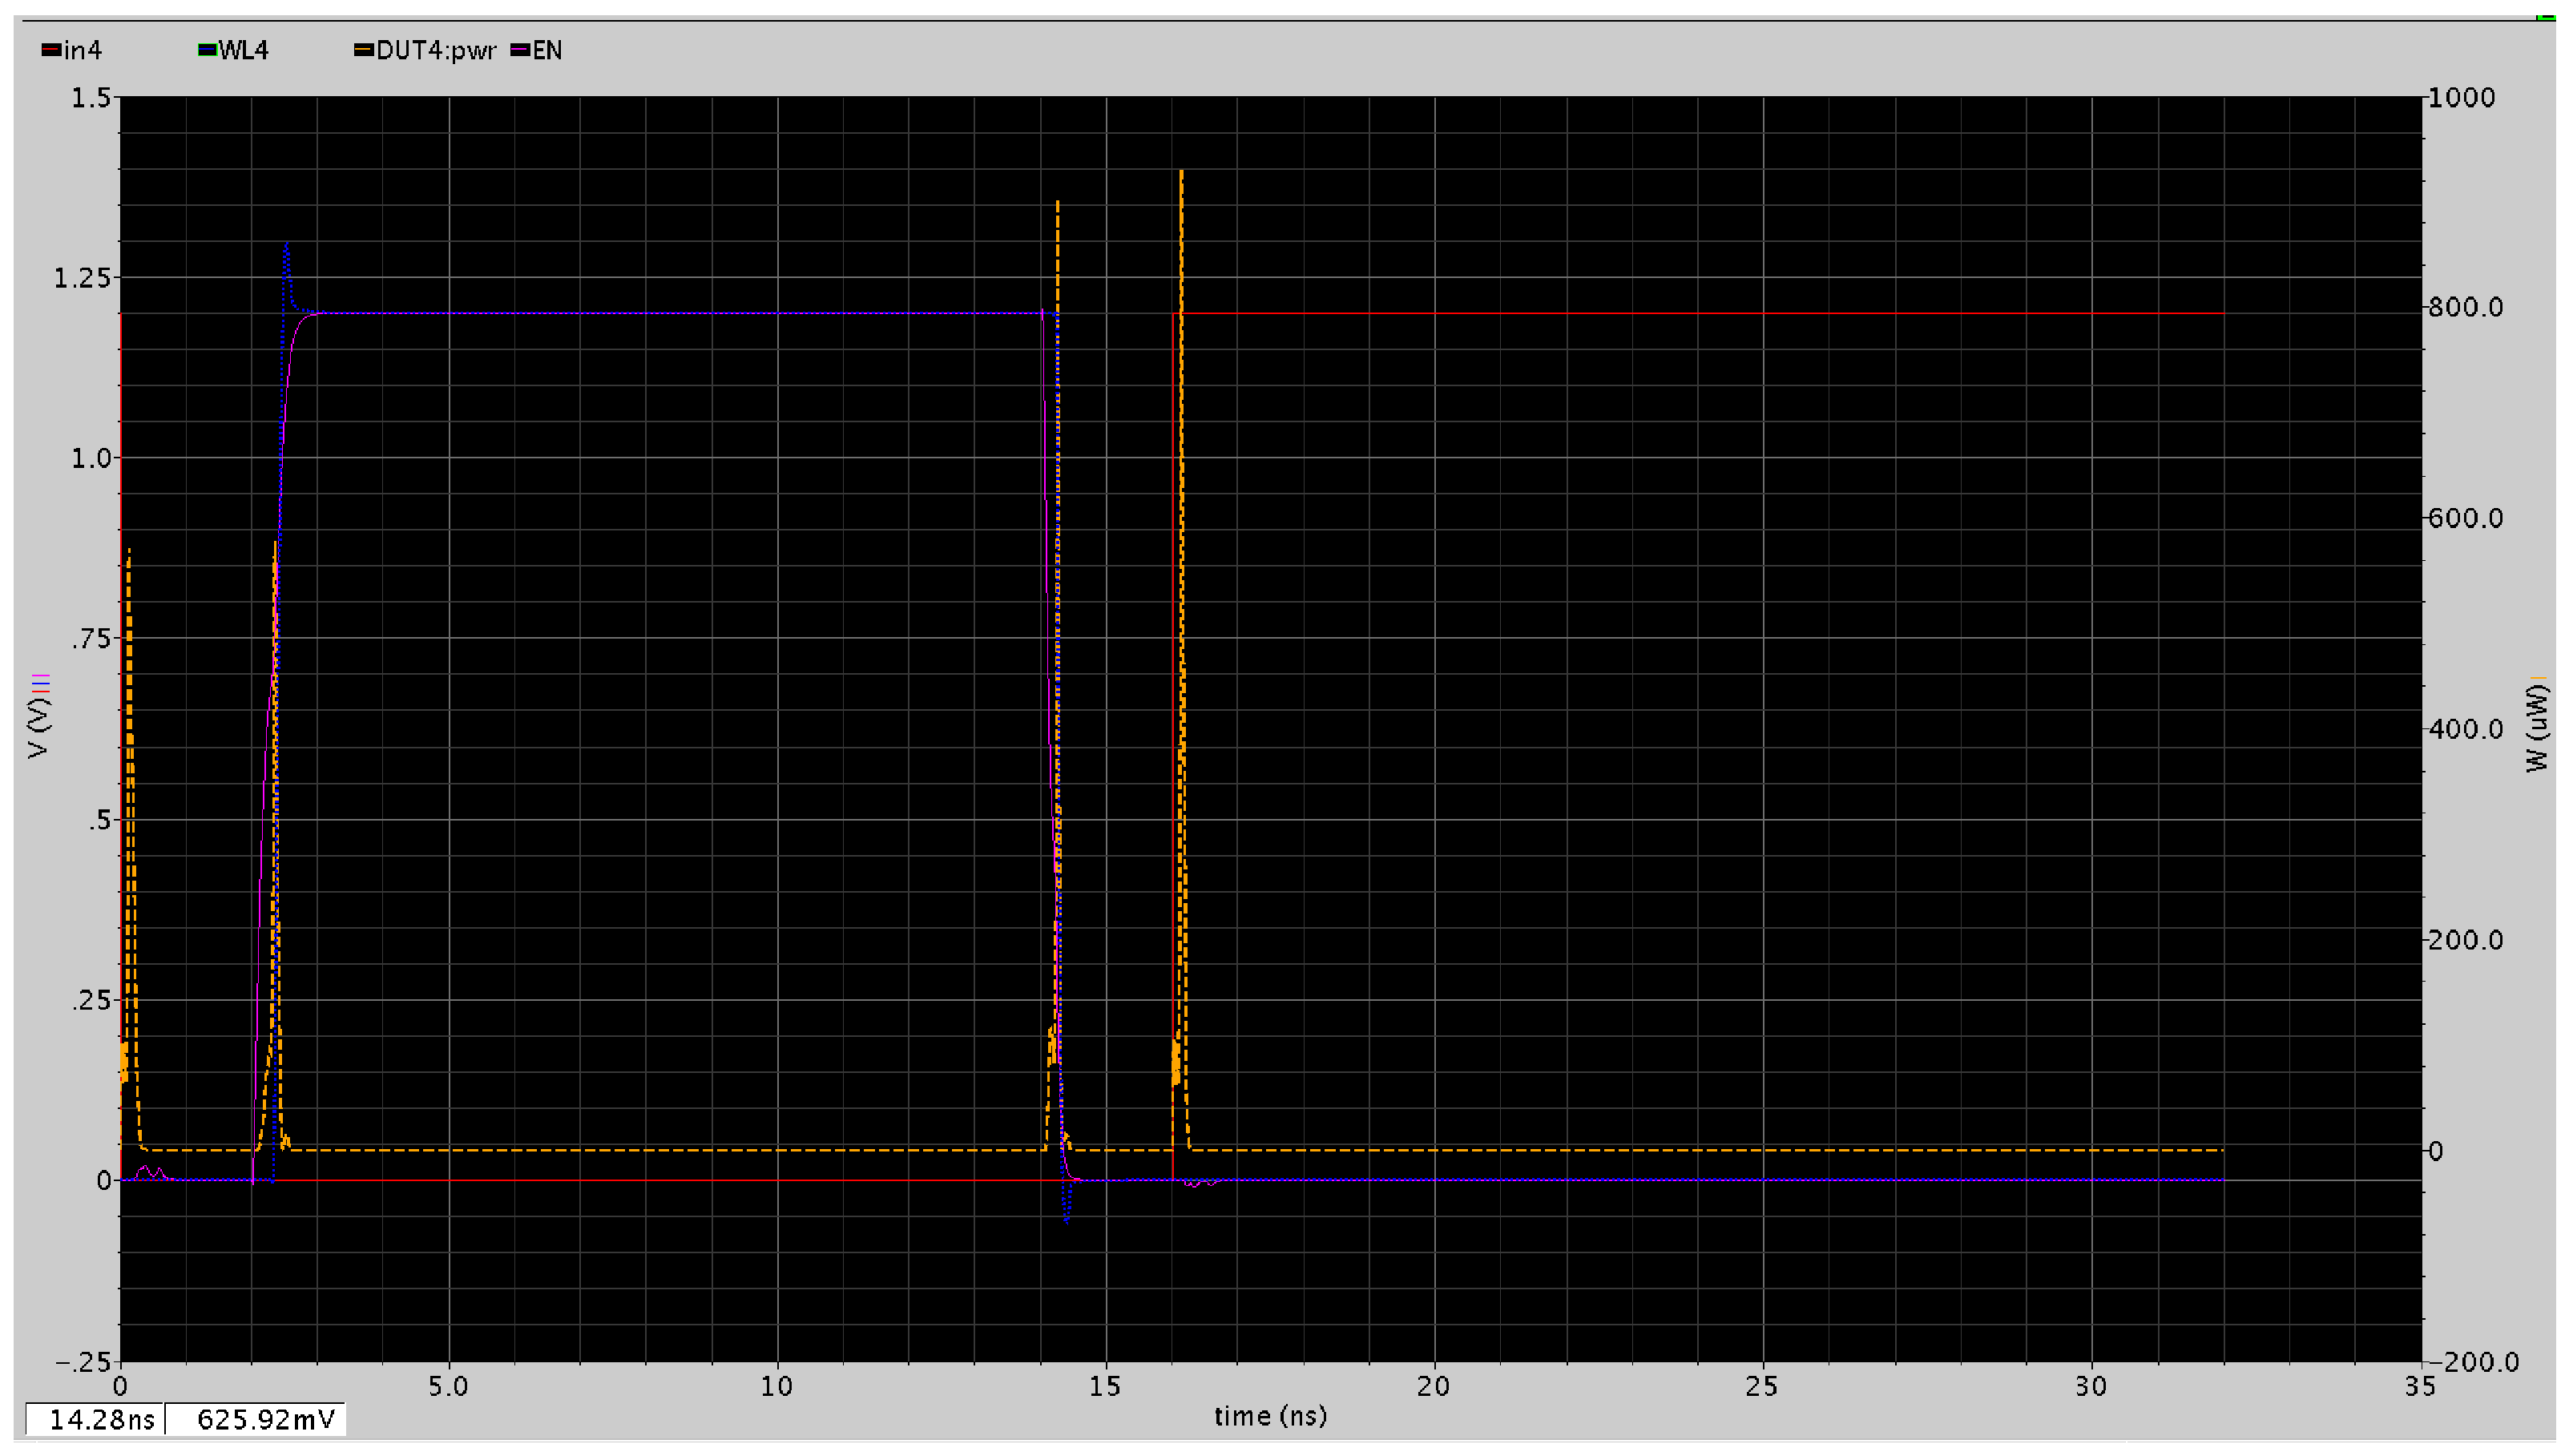
\includegraphics[scale=0.25]{Decoder_power}
\vspace{-5pt}
  \caption{Signals and power waveforms for decoder.}
  \label{fig:decPower1}
\vspace{-5pt}
\end{figure}

\begin{figure}[htb]
  \centering
  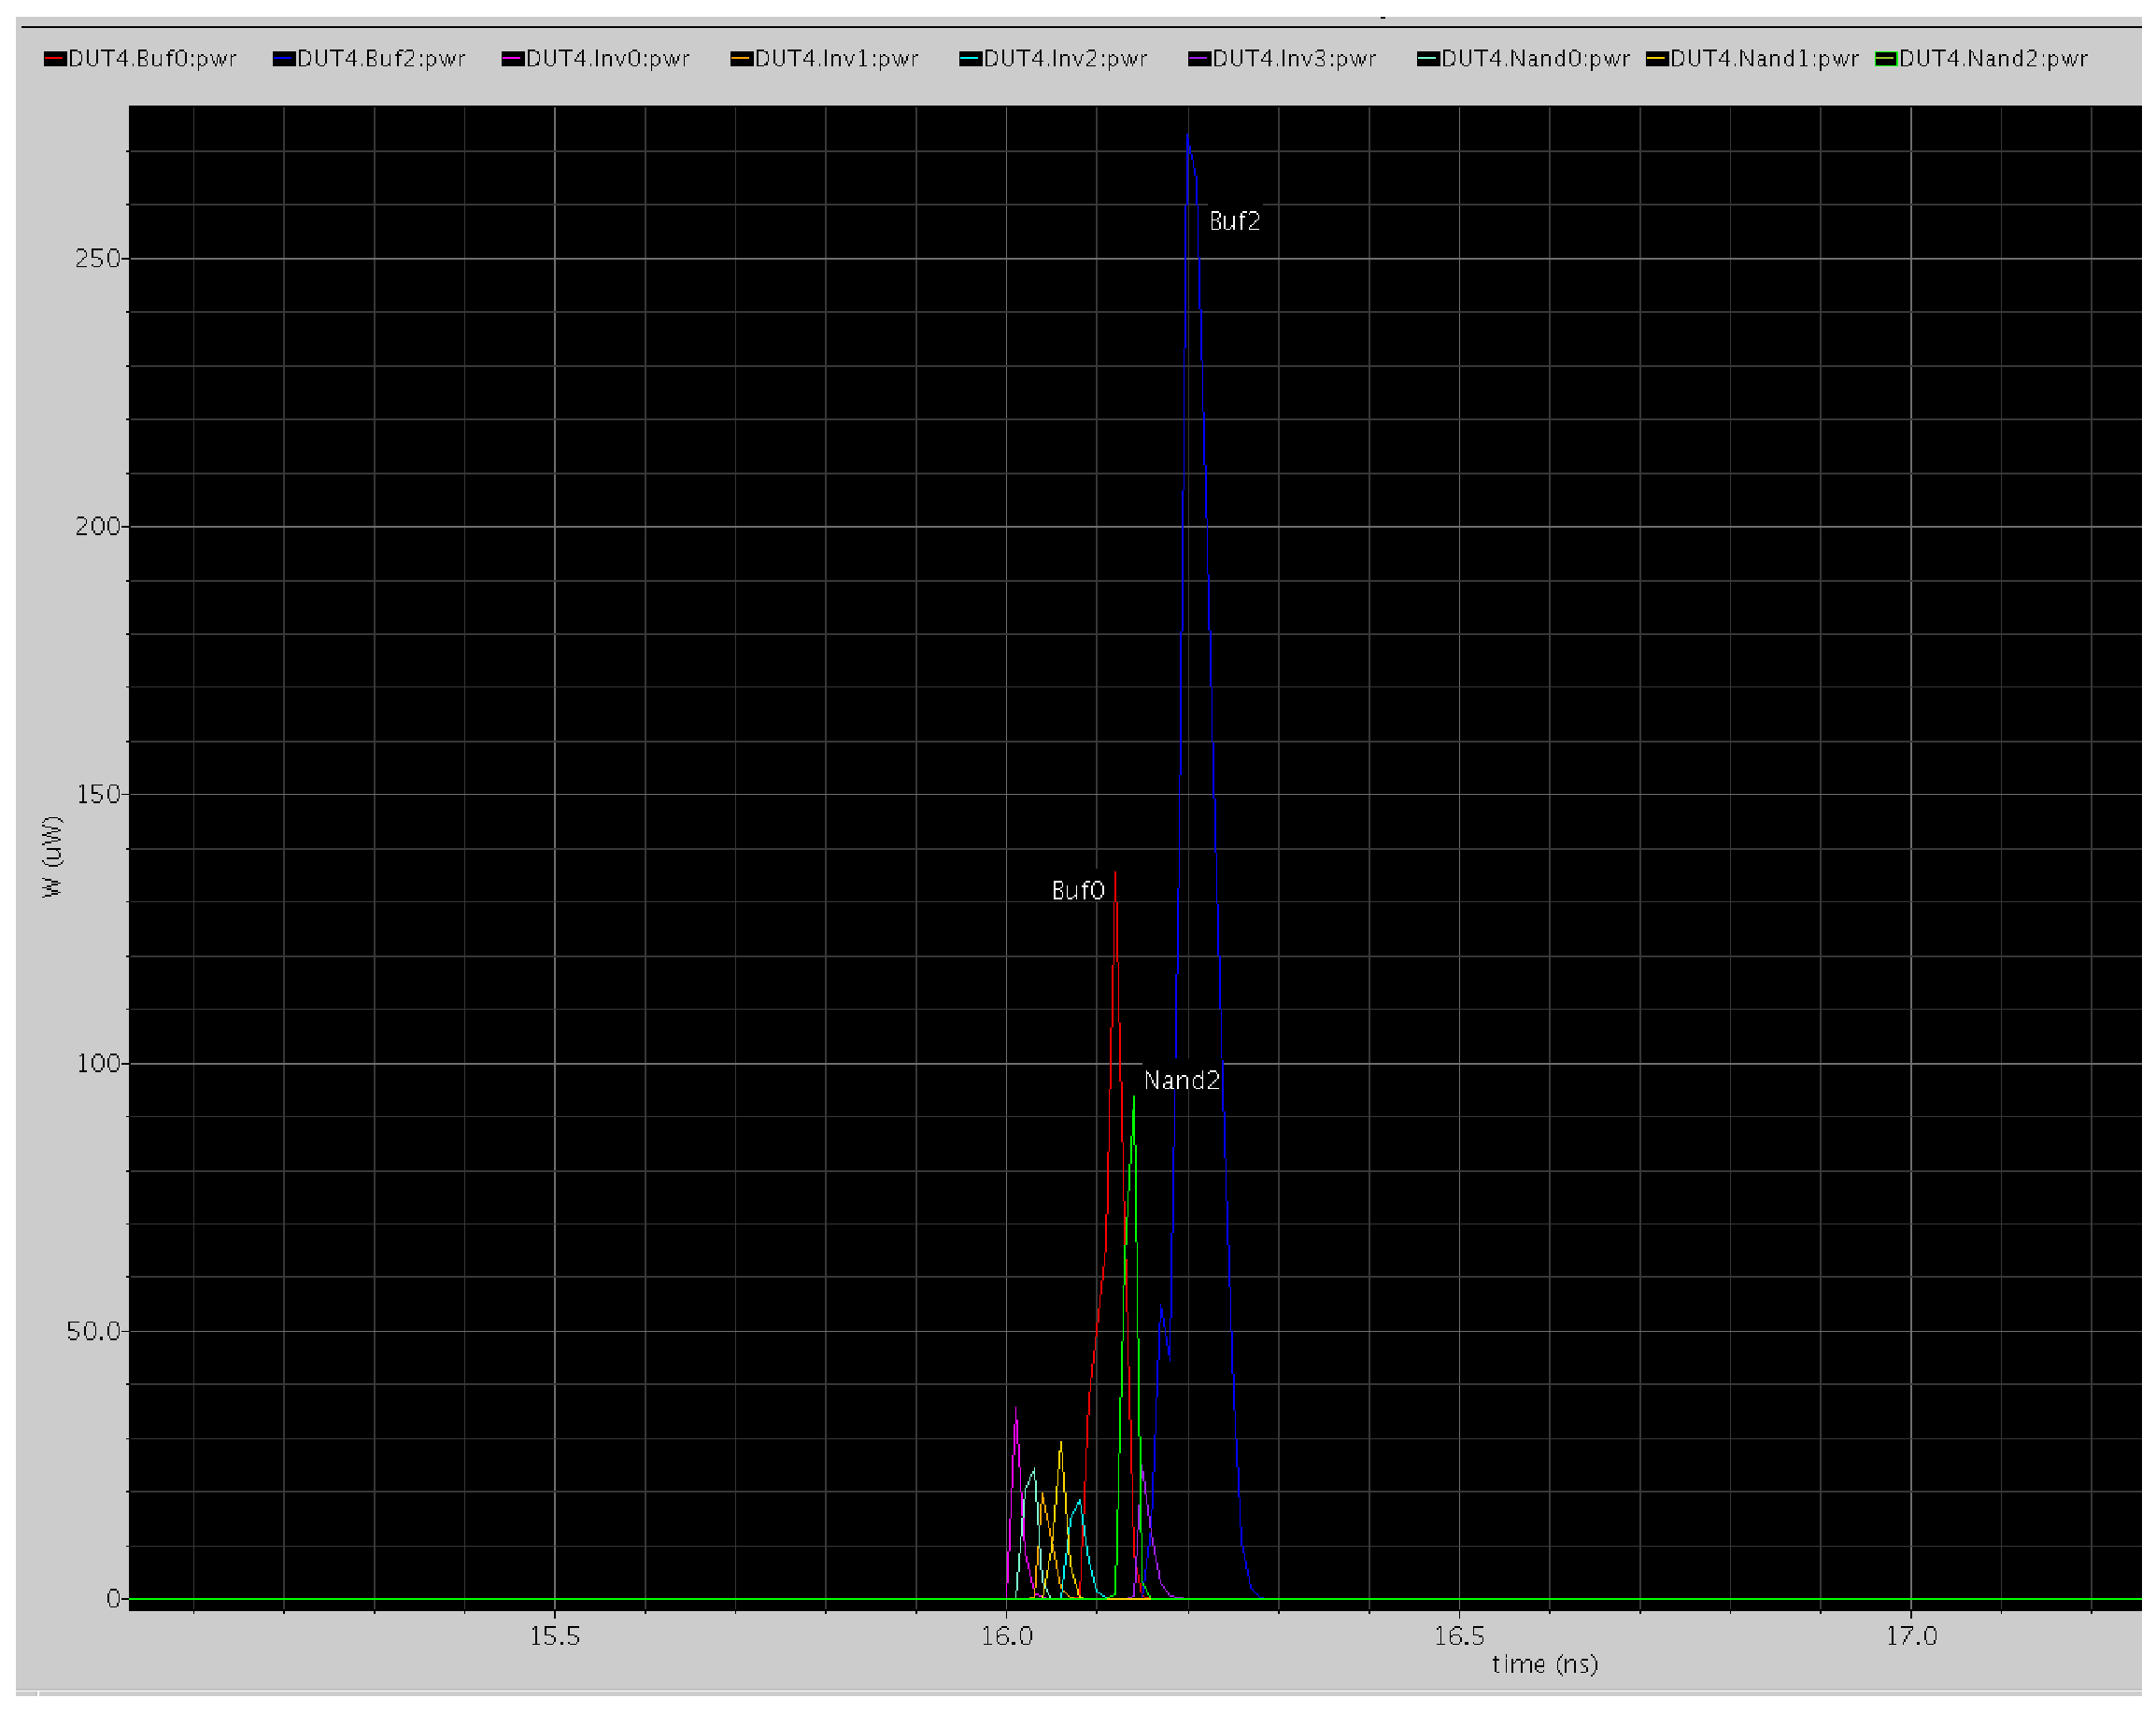
\includegraphics[scale=0.25]{DUT4_3bitdecoder_power}
\vspace{-5pt}
  \caption{Power breakup among gates on the decoder critical path.}
  \label{fig:decPower2}
\vspace{-5pt}
\end{figure}

\subsubsection{Leakage}
Only the leakage of the bitcells is considered. The leakage from VDD and VSS and the BL leakage is added to give the leakage of one cell. This is multiplied with the memory capacity to give the leakage of the array. This slightly overestimates the leakage of the array, since the leakage of the bitcells on the accessed row is counted twice - it was accounted for earlier in the dynamic power measurement for the bitcell.

The total energy can now be summarized by the following equation:
\begin{equation}\label{ewrt}
\displaystyle  E_{WRT}=erowpre+ecoldec+ewld+eiowr*ws+(ecdwr*ws+ecdrd*(cols-ws))+esach*ws+(ebcwr*ws+ebcrd*(cols-ws))+etmng+elkg*capacity
\end{equation} 
where
\begin{description}
\setlength{\itemsep}{0cm}
\setlength{\parskip}{0cm}
\item{\textit{erowpre}} = row-predecode energy
\item{\textit{ecoldec}} = col-decoder energy
\item{\textit{ewld}} = WL driver energy
\item{\textit{eiowr}} = IO energy during write
\item{\textit{ecdwr}} = CD energy during write
\item{\textit{ecdrd}} = CD energy during read
\item{\textit{esach}} = SA input/muxed out BL pre-charge energy
\item{\textit{ebcwr}} = bitcell flip energy
\item{\textit{ebcrd}} = bitcell read energy
\item{\textit{etmngwr}} = timing energy during write
\item{\textit{elkg}} = leakage energy
\end{description}

\subsection{Read}
The read operation can be broken down roughly into four stages(Figure~\ref{fig:rdstg}). The first stage,s1, is the same as in the write (e.g. decode). In s2, the WL goes high and the appropriate BL droops due to cell I$_\text{READ}$. In s3, the SA is enabled once a sufficient differential is developed to resolve the BL differential. In s4, the BLs and the SA inputs are precharged back. s4 can occur in parallel with s1 of the next cycle. In sum, the read operation consists of the following actions.
\begin{enumerate}
\setlength{\itemsep}{0cm}
\setlength{\parskip}{0cm}
\item Input data latching in IO (`io')
\item Row pre-decode (`rowpre')
\item Column decode (`coldec')
\item WL enable (`wld')
\item Bitline droop (`bldr')
\item SA resolution (`sa')
\item Precharge BL/BLB (`cdch')
\item Precharge RDWR/NRDWR (`sach')
\end{enumerate}

\begin{figure}[htb]
  \centering
  
\includegraphics[scale=0.3]{rdStg}
\vspace{-5pt}
  \caption{Stages of the read operation}
  \label{fig:rdstg}
\vspace{-5pt}
\end{figure}

The minimum cycle time for read (T$_\text{MIN-R}$) can be determined as:
\begin{equation}\label{tminr}
\displaystyle  T_{MIN-W}=max(io,rowpre,colpre,cdch,sach) + wld + bldr + sa
\end{equation} 

The setup time for the flip-flop that latches the output of the SA must also be added to this delay. Since that is quite small (Figure~\ref{fig:tsu}) compared to the other terms in equation \ref{tminr}, we ignore it.

\begin{figure}[htb]
  \centering
  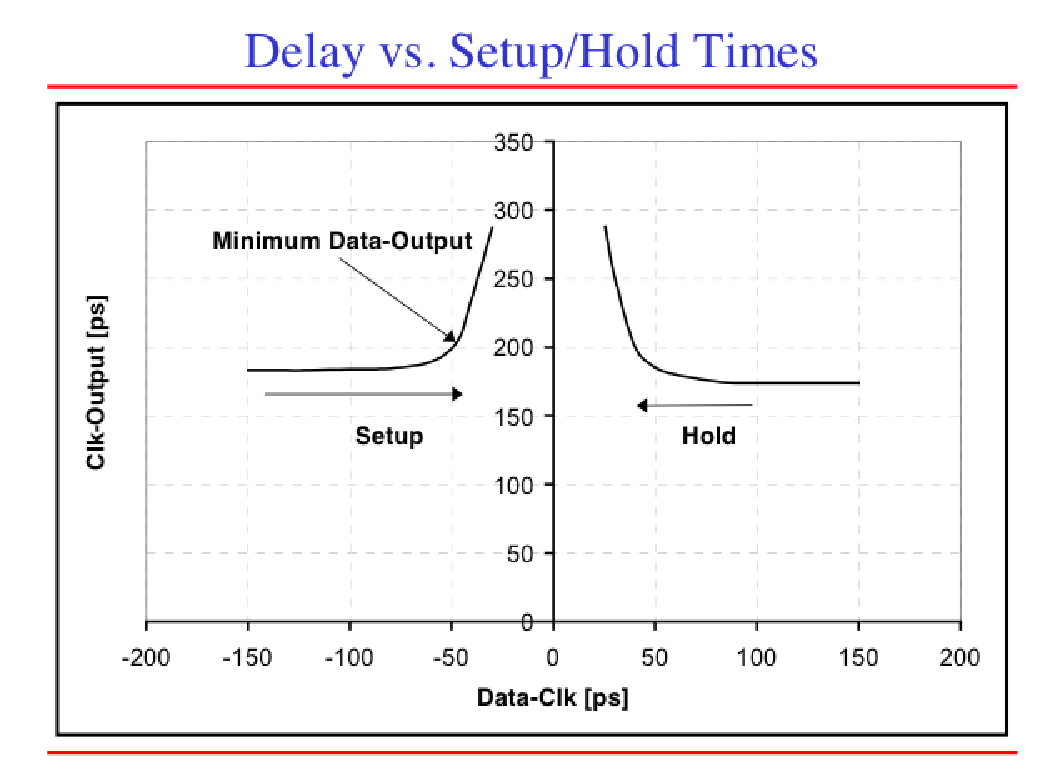
\includegraphics[scale=0.5]{tsu_th}
\vspace{-5pt}
  \caption{Setp and Hold time}
  \label{fig:tsu}
\vspace{-5pt}
\end{figure}

We now discuss the energy components during a read.

\subsubsection{Bitcell}
During a read, the power dissipated through the bitcell is in the PD and PG of the bitcell that are discharging the BL, as shown in Figure~\ref{fig:read_bccd}. 
\begin{figure}[htb]
  \centering
  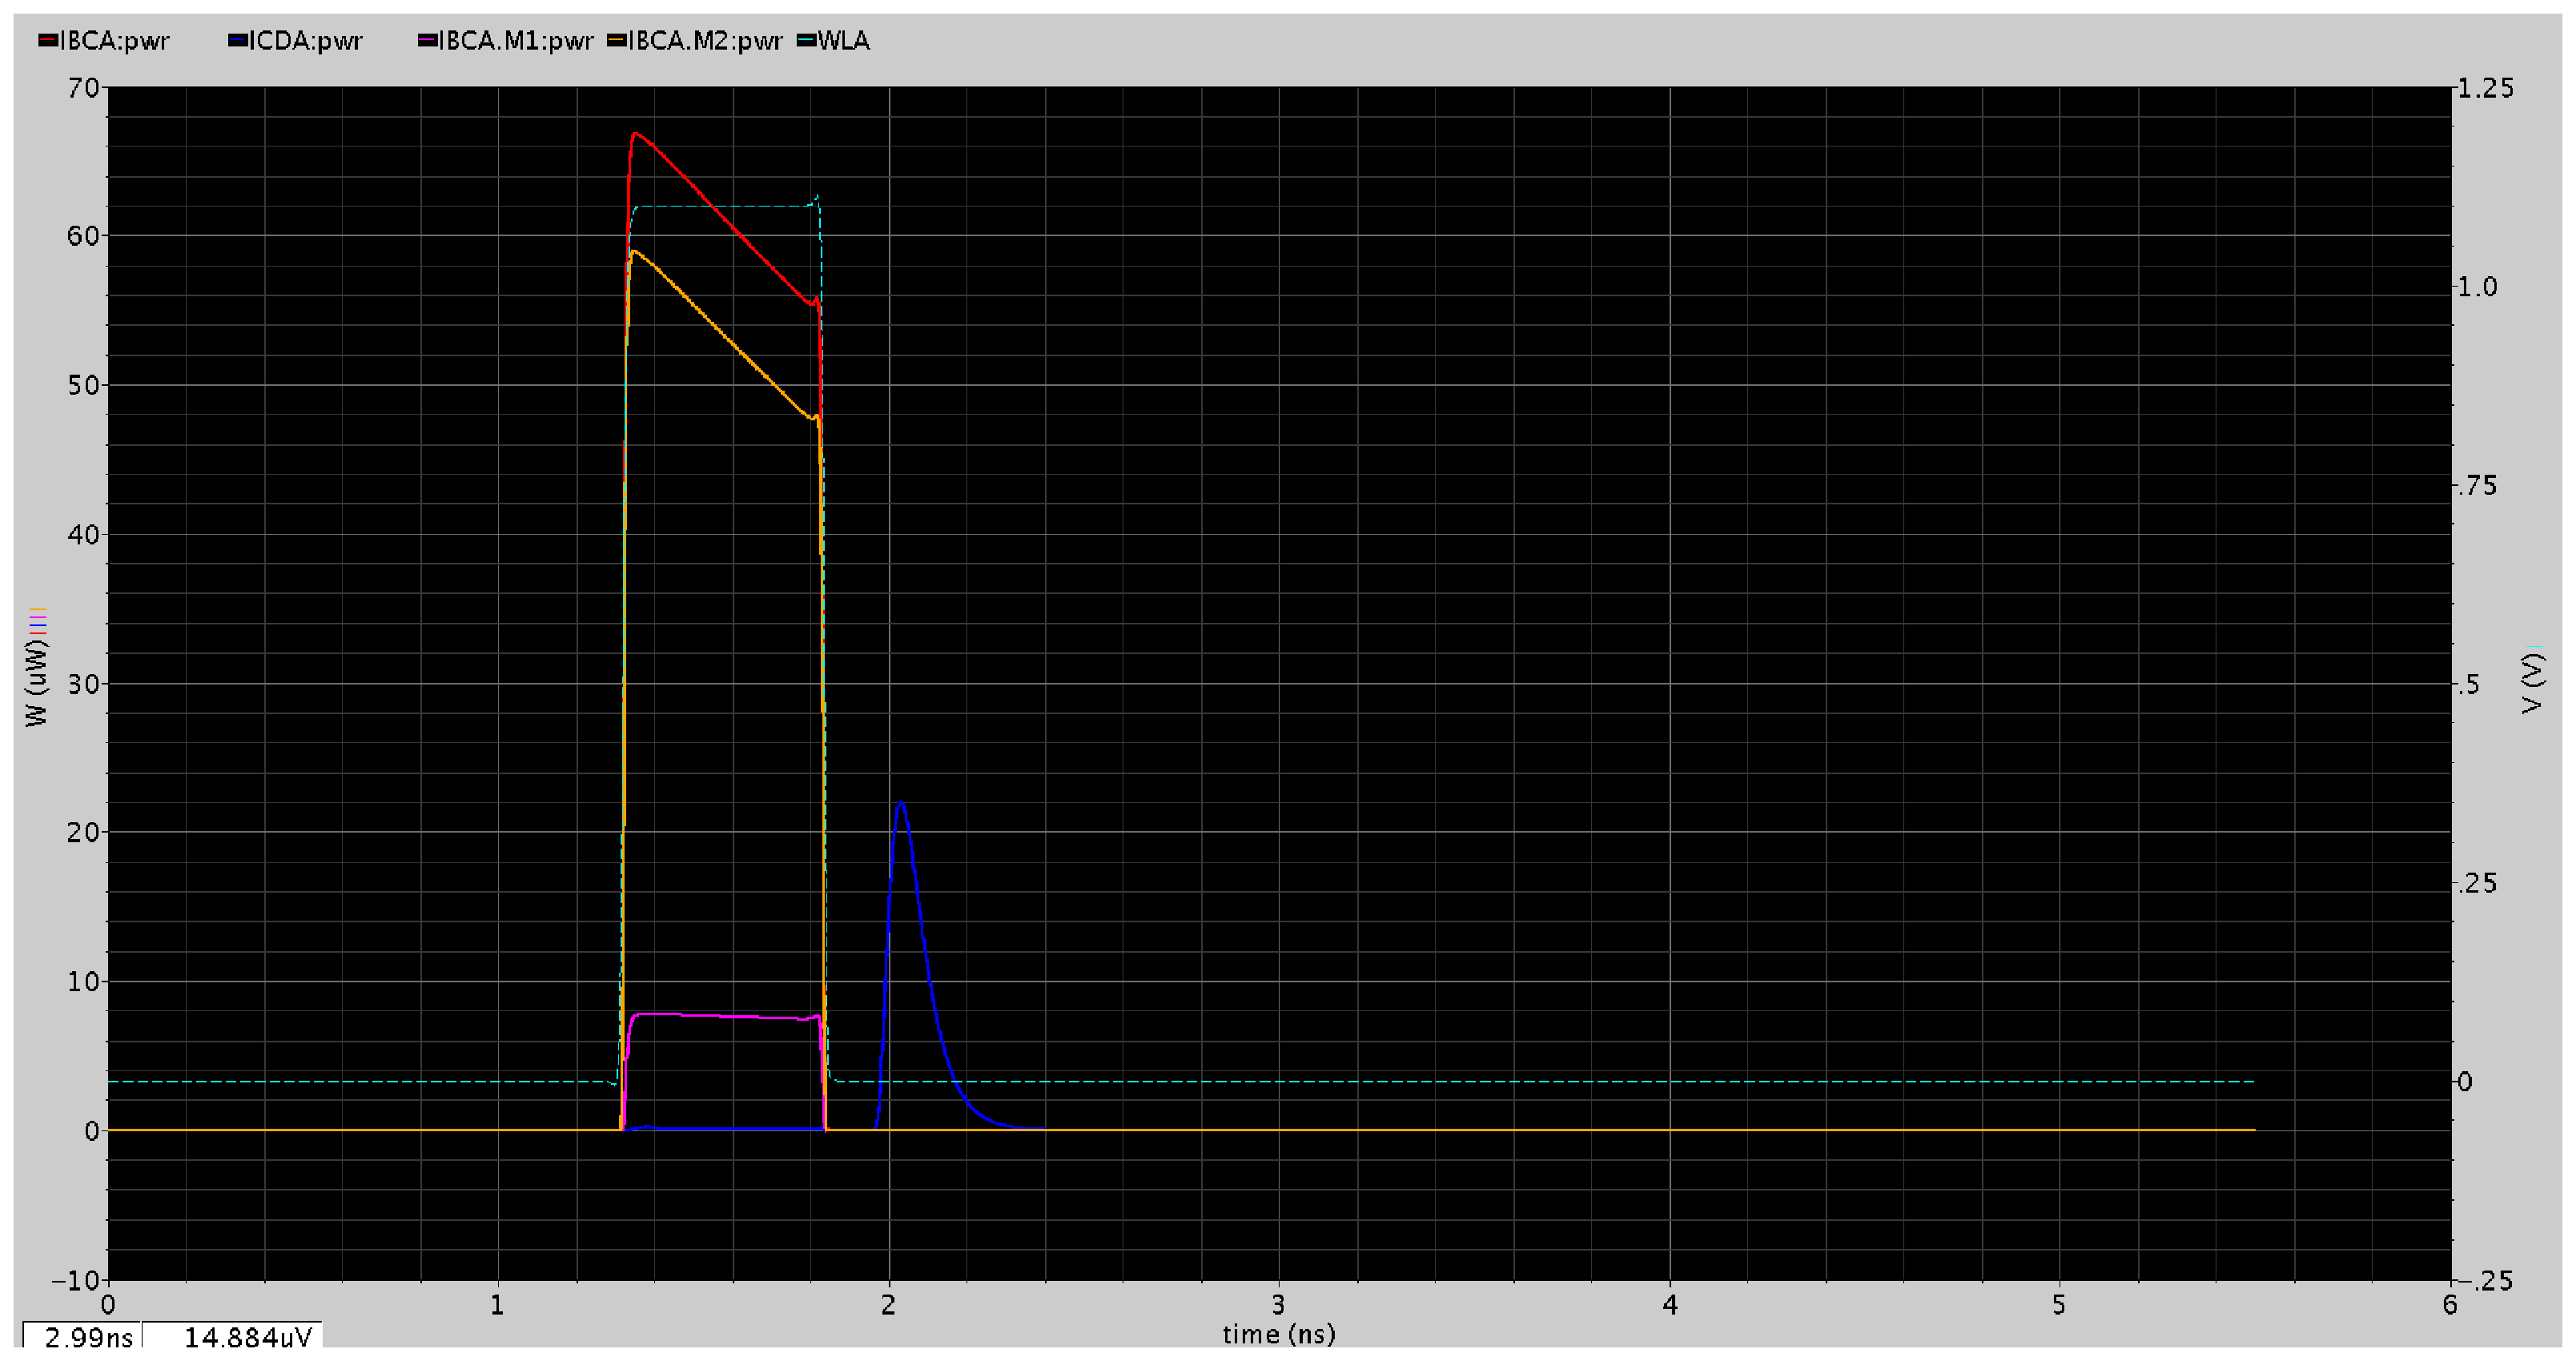
\includegraphics[scale=0.25]{BC_CD_Read_ptm65}
\vspace{-5pt}
  \caption{Signals and power waveforms for CD and bitcell power during read.}
  \label{fig:read_bccd}
\vspace{-5pt}
\end{figure}

\subsubsection{CD}
During a read, the power dissipation in the CD is only due to the precharging of the partly discharged BL back to full rail V$_\text{DD}$, as can be seen in Figure~\ref{fig:read_bccd}. Unlike in the write operation, there is no significant power dissipation in the CD at the beginning of the WL pulse since both the BL and the RDWR/NRDWR nodes are precharged high and there is no significant current through the column-mux transmission gates.

\subsubsection{SA}
There are two main power dissipation sources in the SA during a read, as observed from the waveforms in Figure~\ref{fig:read_sa}. The first component is due to the resolution of the BL differential by the SA. The second part is due to the pre-charging of the SA inputs(e.g. RDWR/NRDWR nodes).

\begin{figure}[htb]
  \centering
  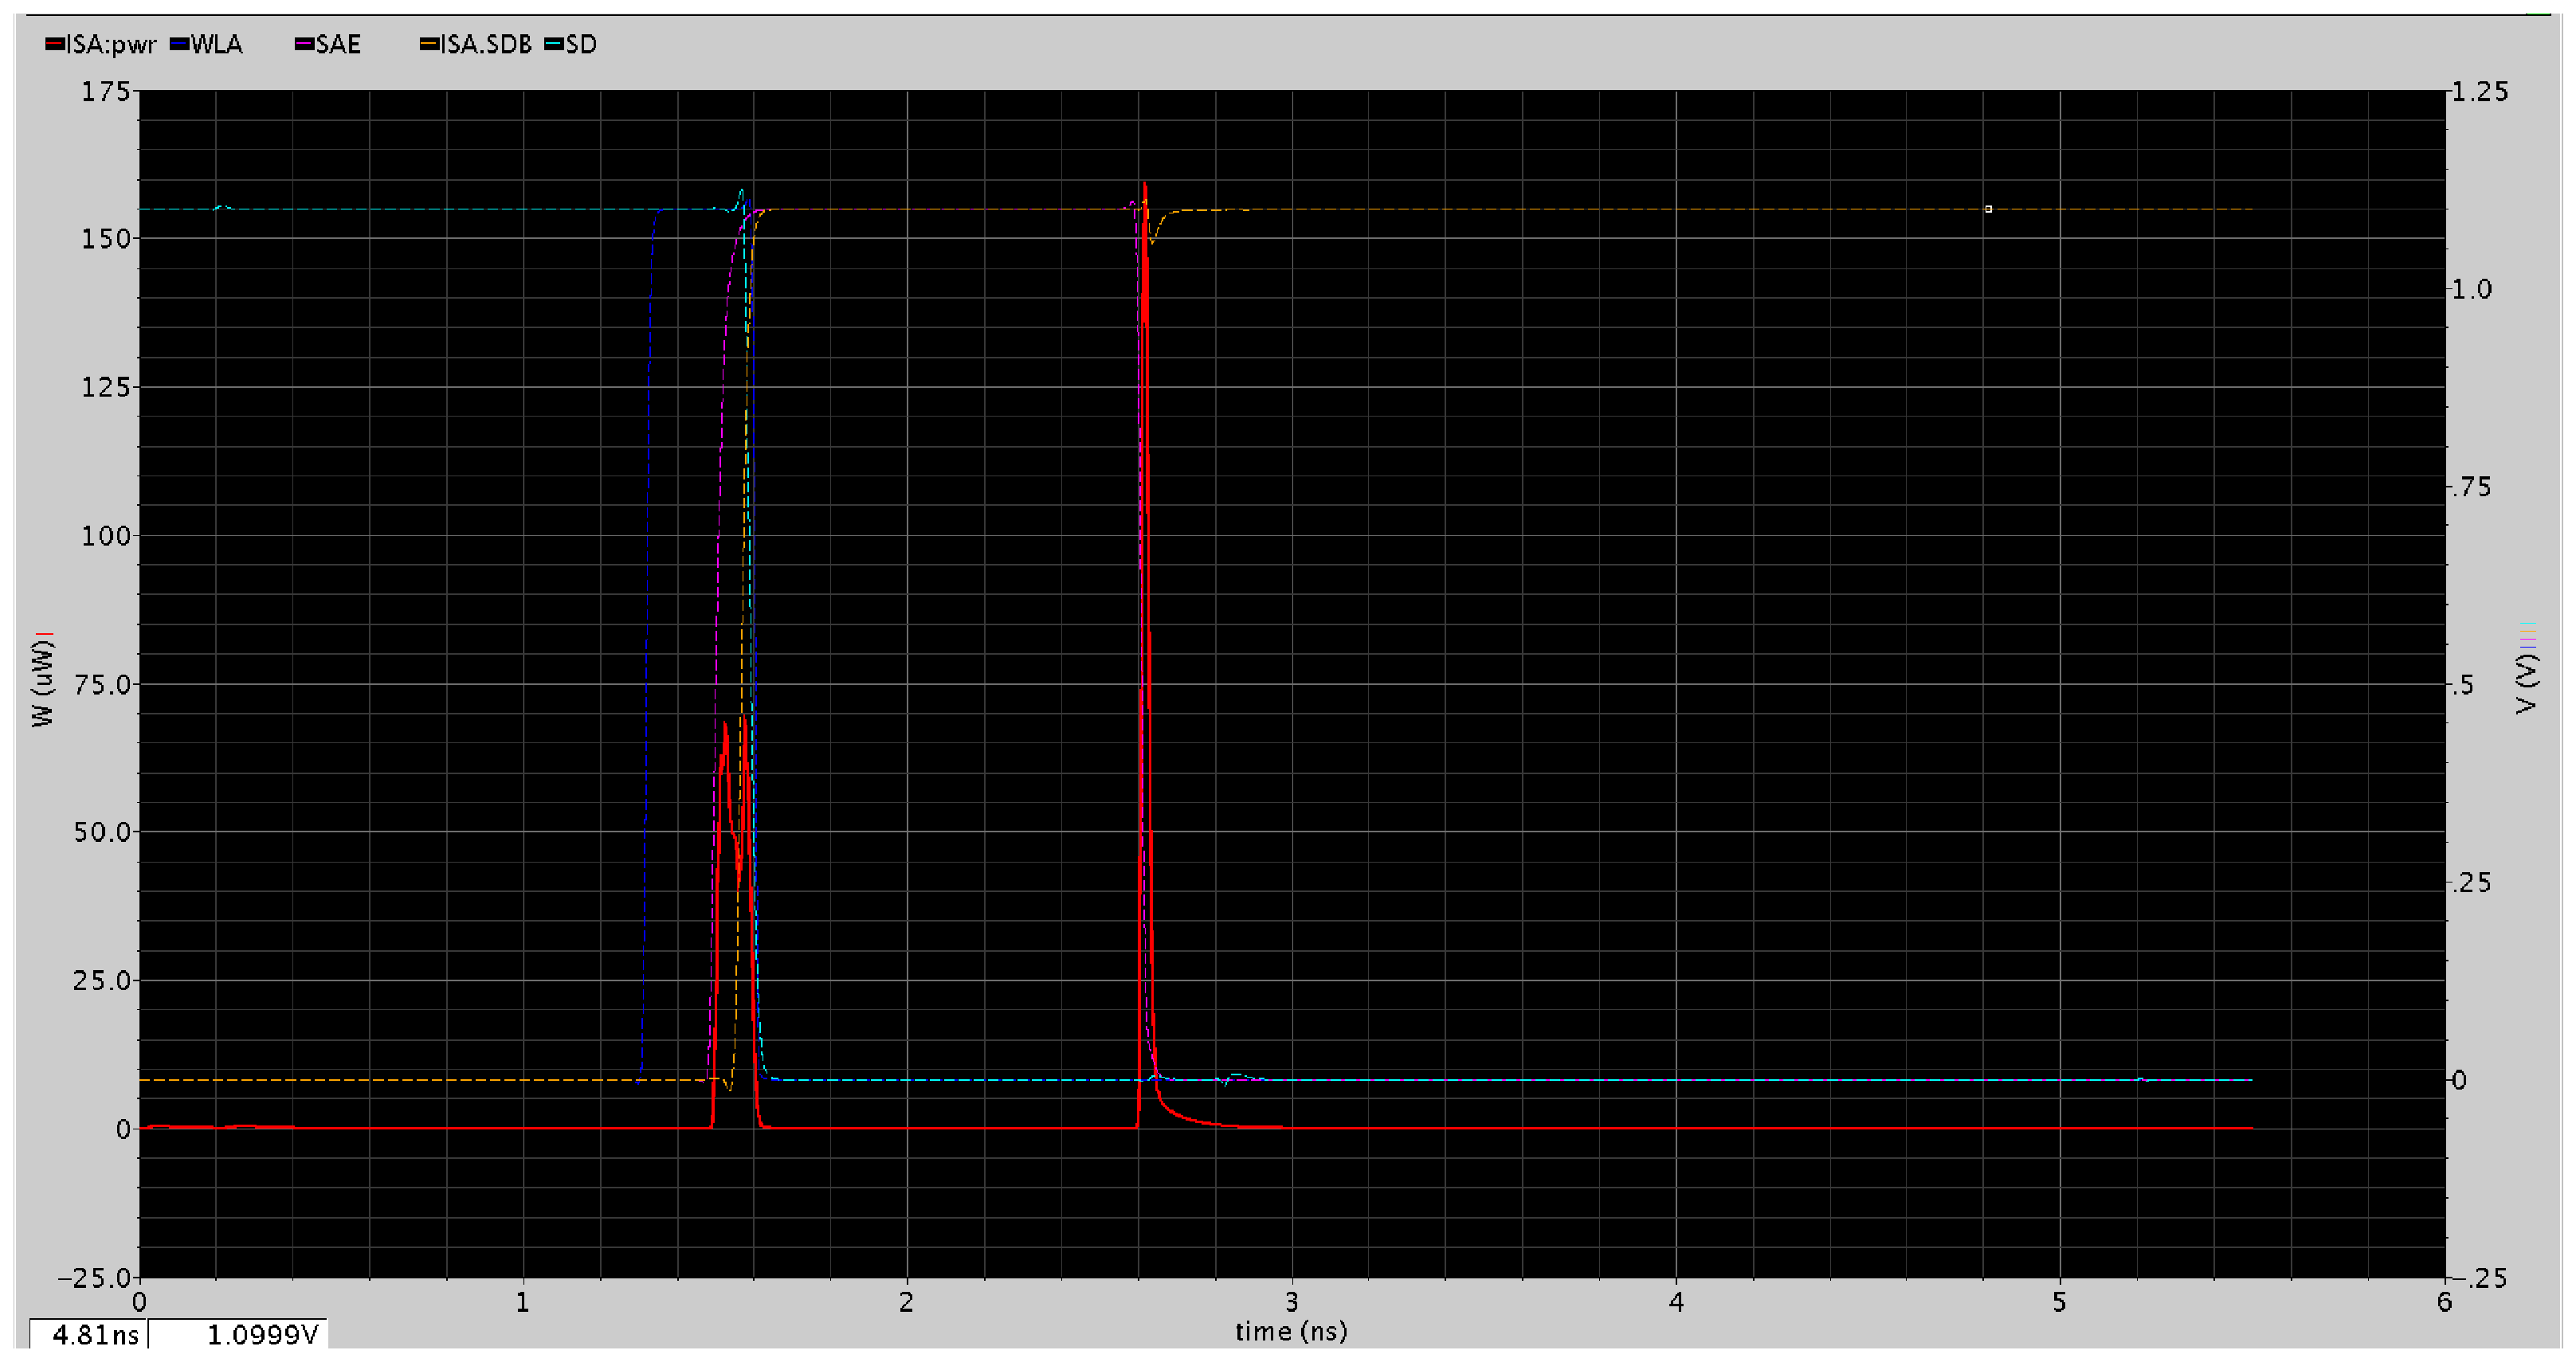
\includegraphics[scale=0.25]{SA_Read_ptm65}
\vspace{-5pt}
  \caption{Signals and power waveforms for SA power during read.}
  \label{fig:read_sa}
\vspace{-5pt}
\end{figure}

\subsubsection{IO}
During a read, the IO power dissipation is predominantly due to the DFFs since the the write drivers are inactive. There are two power consumption events as seen from Figure~\ref{fig:read_io}. These correspond to the rising and falling edges of the clock during which the DFFs consume power. The latching of the SA output data also occurs at the rising edge adding to the power consumption.

\begin{figure}[htb]
  \centering
  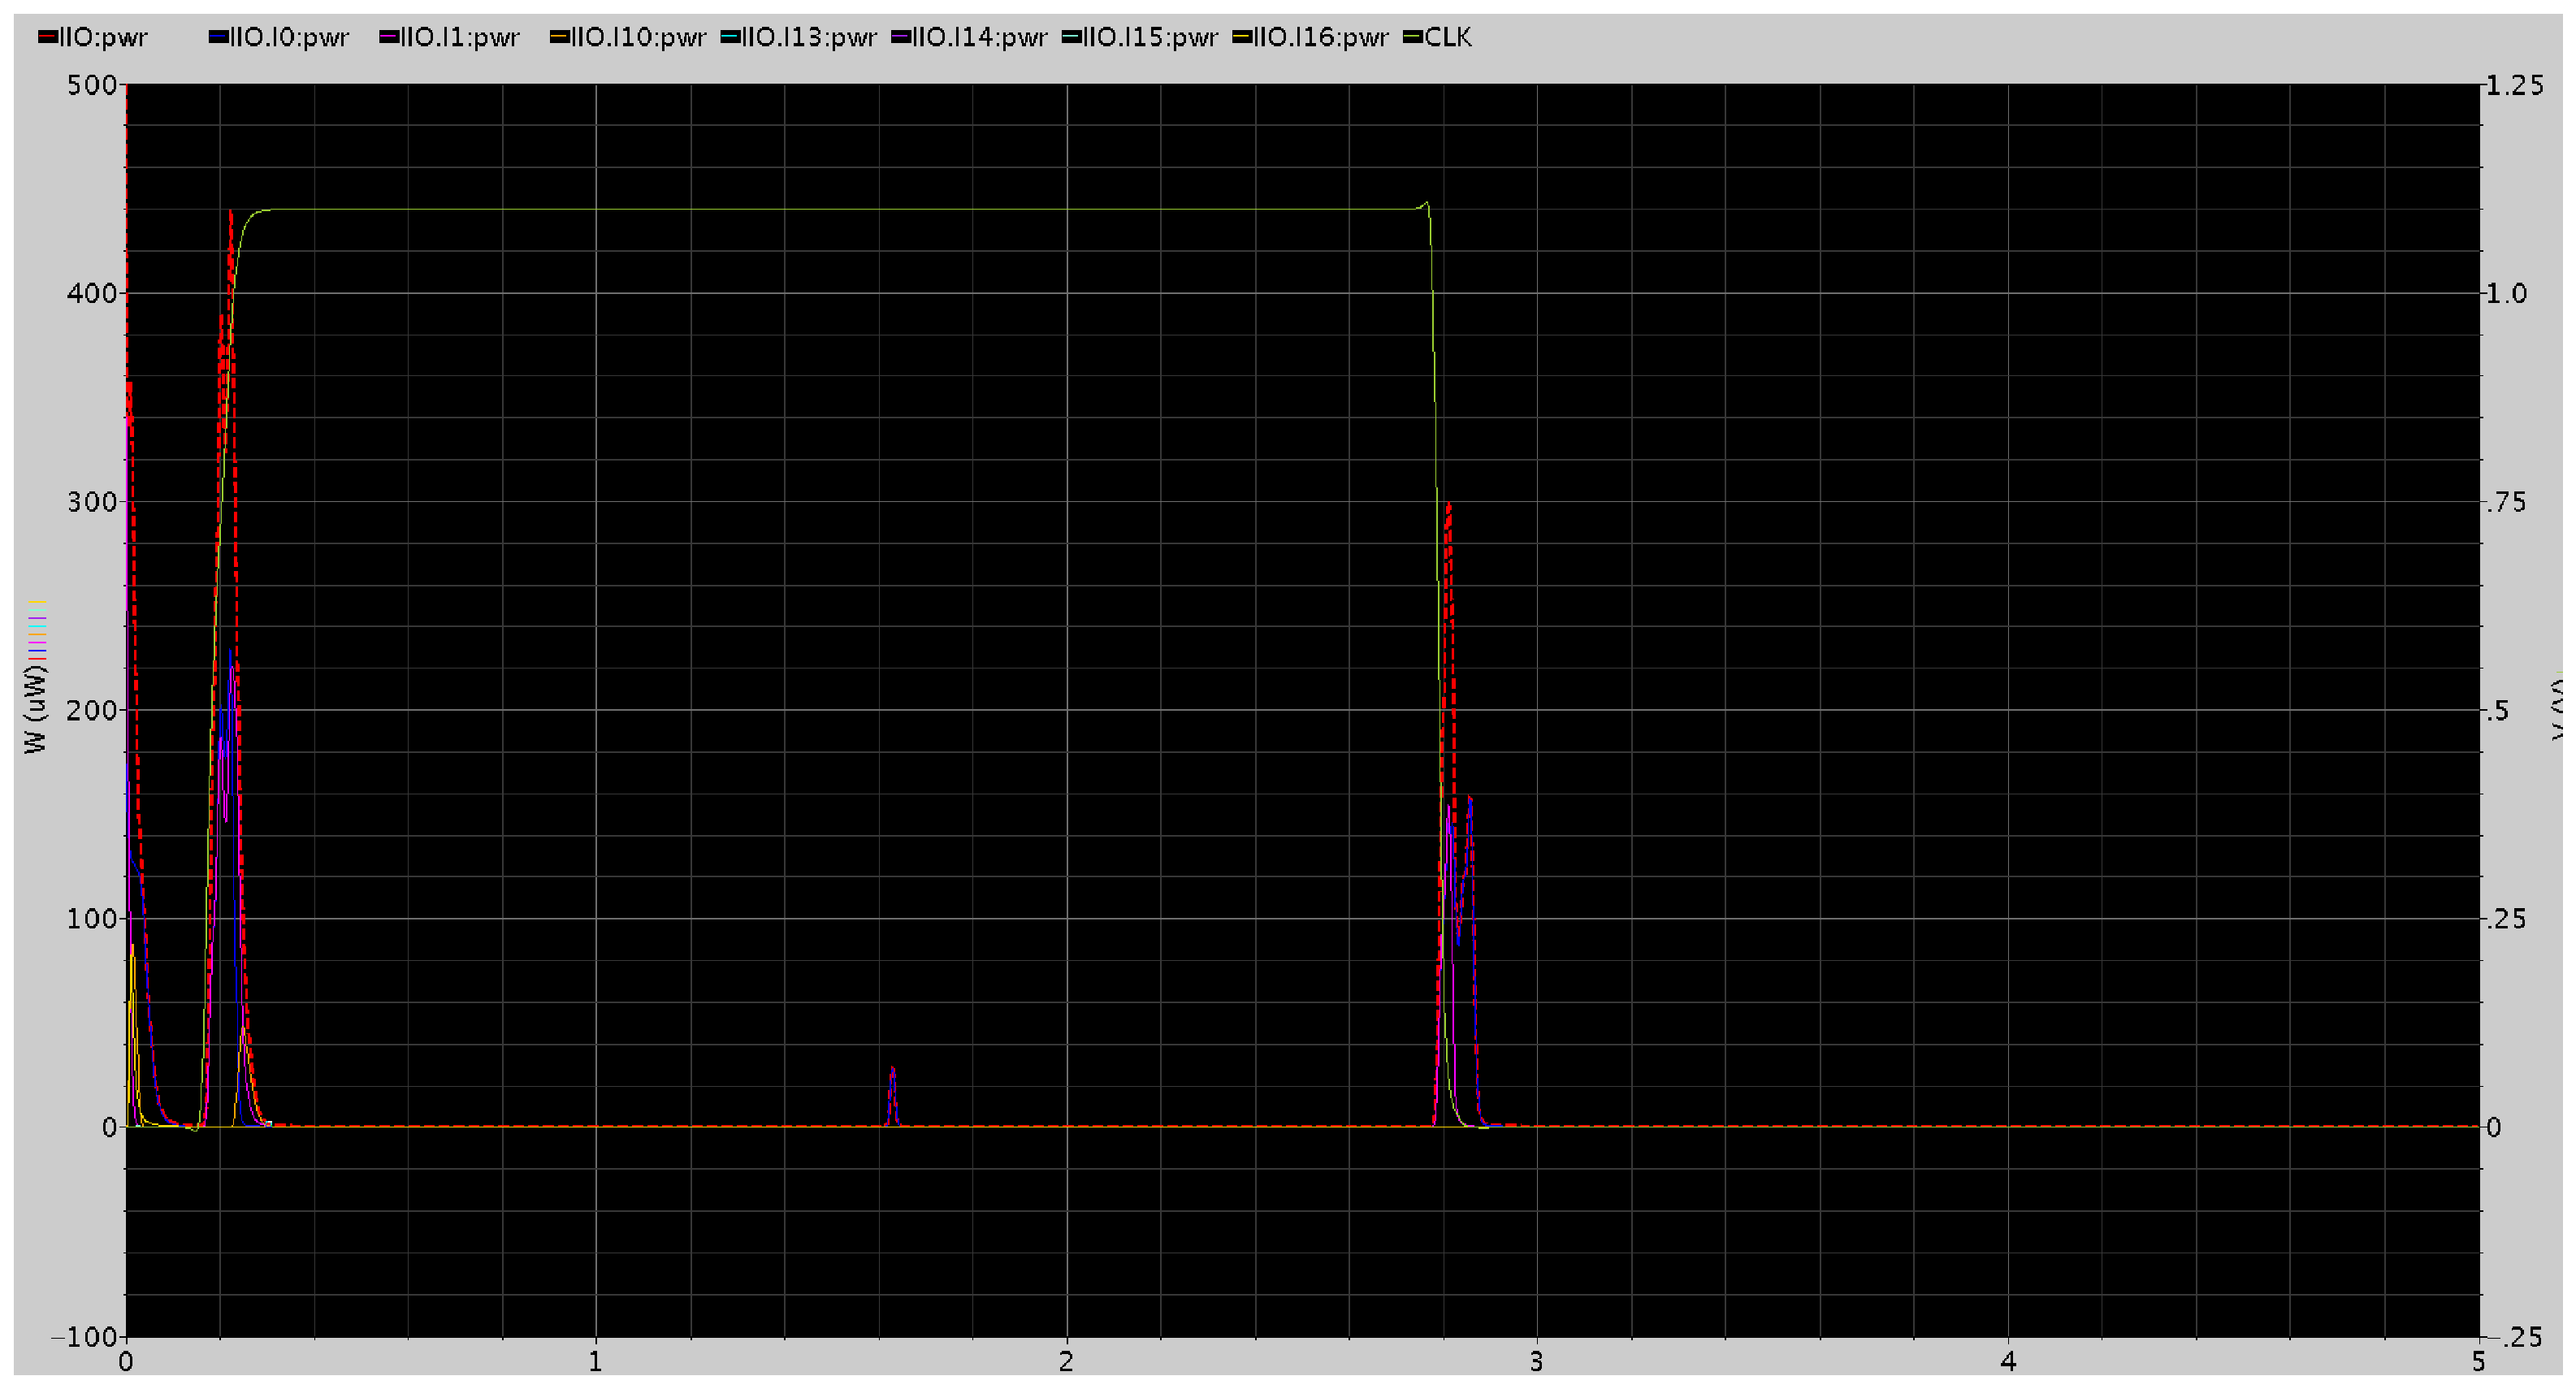
\includegraphics[scale=0.25]{IO_Read_ptm65}
\vspace{-5pt}
  \caption{Signals and power waveforms for IO power during read.}
  \label{fig:read_io}
\vspace{-5pt}
\end{figure}

\subsubsection{Decoder, Timing, Leakage}
The Decoder power consumption and the leakage are the same during write and read and is as described earlier. A single timing block characterization is used to calculate the average power for both read and write as described earlier.

To get the total energy for the IO,CD,SA, and bitcell, we multiply the energy measured from the TASE sim with the word-size as before. The energy per read access can be calculated as:
\begin{equation}\label{erd}
\displaystyle  E_{RD} = erowpre + ecoldec + ewld + eior + ecdrd + esa + ebcrd + etmngrd + elkg
\end{equation} 

\begin{description}
\setlength{\itemsep}{0cm}
\setlength{\parskip}{0cm}
\item{\textit{esa}} = SA energy during read
\item{\textit{etmngrd}} = Timing energy during read
\item{\textit{eior}} = IO energy during read
\end{description}
